\newpage
\section{Regions of interest}
\label{sec:MBSR}
%\minitoc
For a given selection in $\HT$ and $\LT$, the plane $\njet$ vs. $\DF$ is divided in 4 kinematic regions.
The bins at low and high $\DF$ are called control region~(CR) and signal region~(SR), respectively.
The low and high $\njet$ bins are called sideband~(SB) and mainband~(MB), respectively.
A sketch of the regions is shown in Fig.~\ref{fig:regions}. In this section, SR, CR, MBs are defined. SBs are designed to measure transfer factor from CR to SR for data driven background estimation. SBs are described in Ch.~\ref{chap:Rcs} when background estimation is discussed.
\begin{figure}
\label{fig:regions}
    \centering
    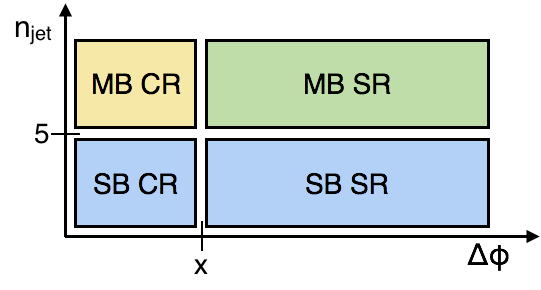
\includegraphics[width=0.7 \textwidth]{PhD_Thesis_v4/Plots/analysis/signalRegions/Regions.png}
    \caption[Sketch of the $\njet$ vs. $\DF$ plane]{The $\njet$ vs. $\DF$ plane for SR, CR, MB, SB.}
    \label{fig:my_label}
\end{figure}
\subsection{Signal and control region}
SRs are defined based on the expected deviation from the SM under a SUSY signal hypothesis. Fig.~\ref{fig:DF} shows the main search variable $\DF$ after the baseline selection. The plot shows that the SM background processes peak at zero while the signal models are almost flat. This shape difference suggests high values of $\DF$ for SR and the low values as CR, which are used in the background estimation. It can also be seen from the distribution that after the baseline selection, $\wJets$ and $\ttJets$ are the main background components. The $\ttbar$ composition in the CR is dominated by the single leptonic decays while in the SR the di-leptonic  $\ttbar$ decays are dominating.
 \begin{figure*}[!hbt]
    \begin{center}
 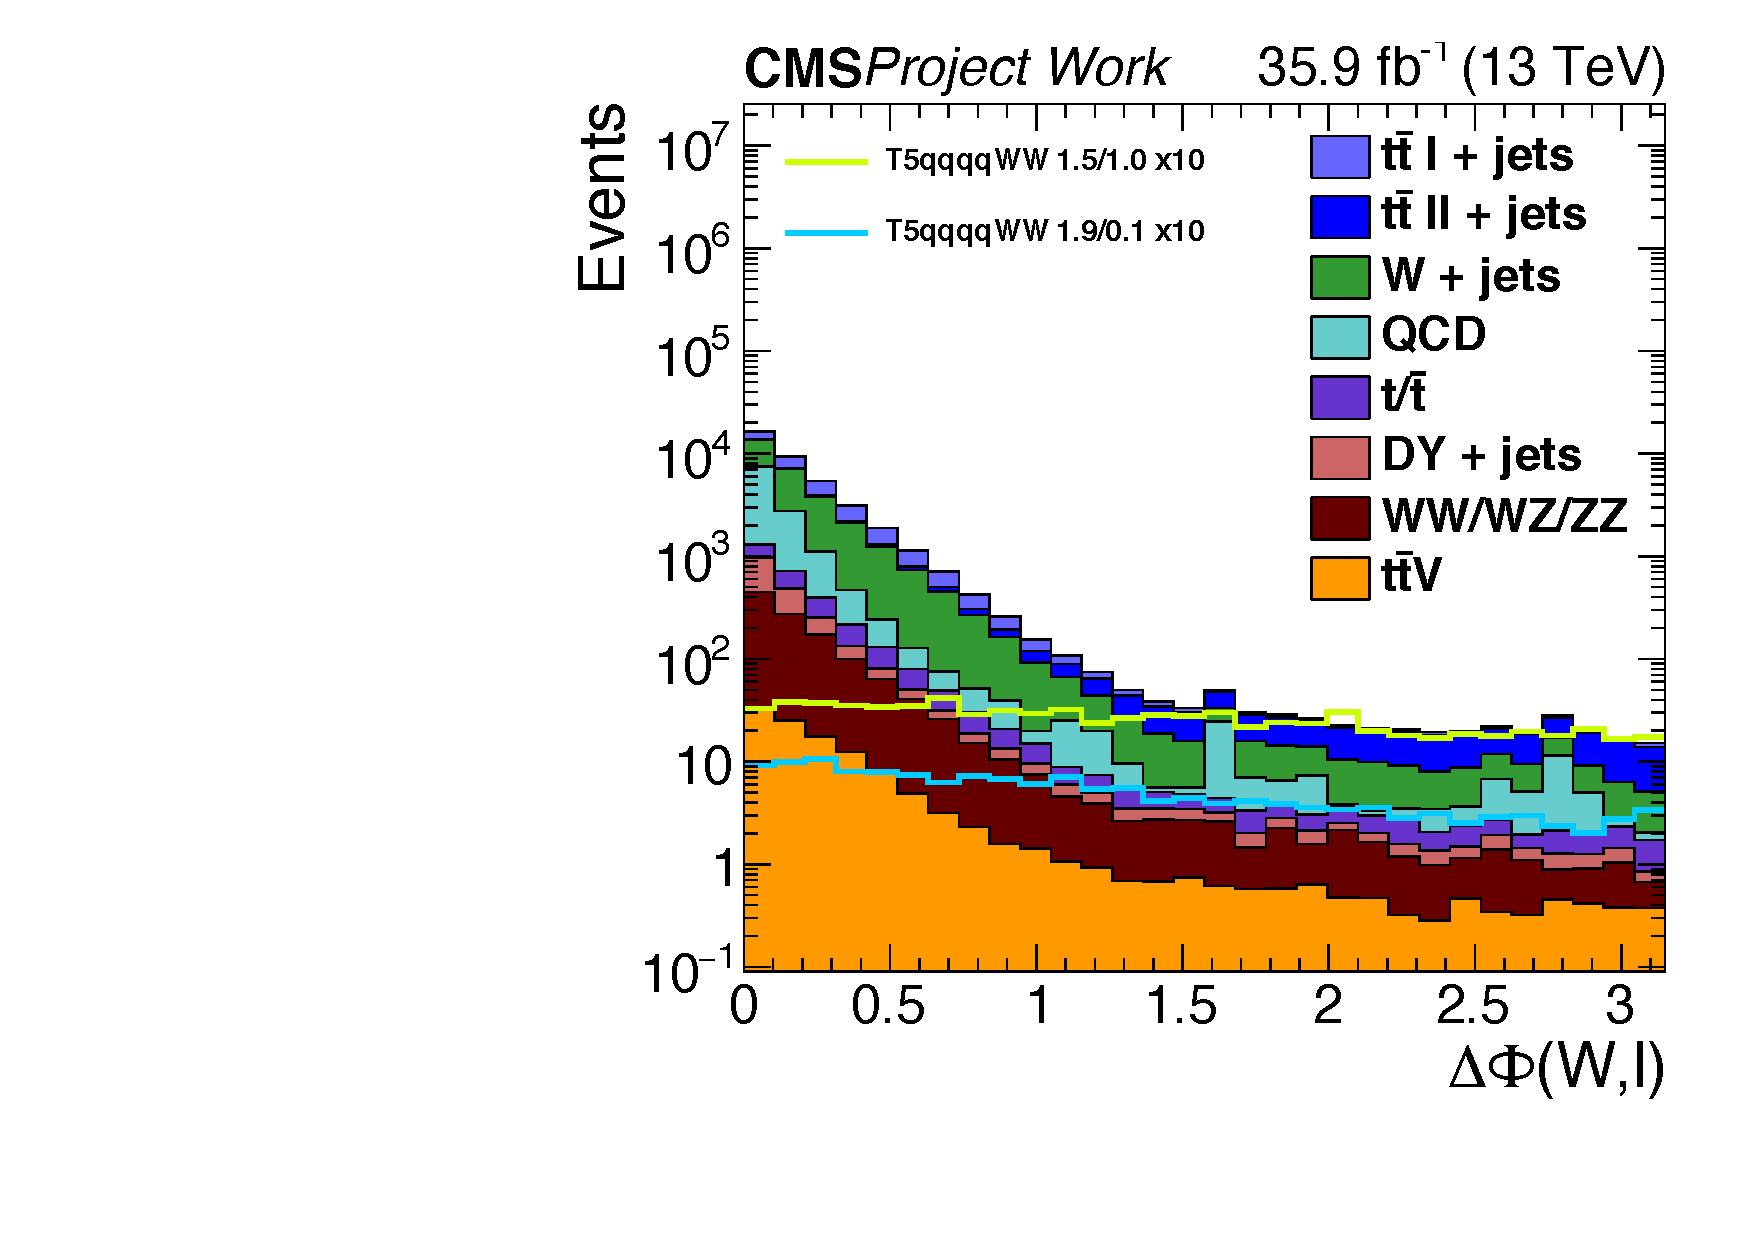
\includegraphics[width=0.5 \textwidth]{Plots/analysis/signalRegions/deltaPhi_Wl_narrownormal}
  \caption[The $\DF$, after the baseline selection, MC only]{ \label{fig:DF} The $\DF$, after the baseline selection, requiring at least five jets and non of b-tagged, minimum $\HT$ of 500 GeV, a minimum $\LT$ of 250 GeV and exactly one lepton (electron of muon) with $\pt >$25 GeV. The simulated background events are stacked on top of each other, and several signal points are overlaid for illustration without being stacked.
  }
   \end{center}
\end{figure*}
\subsection{Mainband regions}
Mainband regions are exclusive kinematic regions defined according to $\njet$, $\HT$ and $\LT$. These regions are designed to further increase the sensitivity to a range of different gluino and neutralino mass scenarios.\\
%The binning is designed for an integrated luminosity of 40~fb$^{-1}$. 
First, the phase space after baseline selection is subdivided into three jet multiplicity bins: $\njet=5$, $6\leq\njet\leq7$, $\njet\geq8$. As shown in Fig.~\ref{fig:signalKin}, signal model with a lower mass gap has a peak in lower $\LT$ and $\HT$ values than the higher mass gap signal model. Therefore, further binning is introduced in $\LT$ and $\HT$. To determine the binning, high sensitivity is considered. A profiled likelihood analysis is performed to measure the sensitivity. Additionally, to have a robust background estimation, the expected yield of background MC for each bin is required to be at least 0.5.\\
%requiring the simulated total background yield at least 0.5 event in each MB SR.   the bins with the highest figure of merit are chosen among a spectrum of bins.
%Then, a profiled likelihood analysis is performed for several combination. Additionally, to have robust background estimation, the expected yield of background MC for each bin is required to be at least 0.5. The bin combination with the highest sensitivity is chosen to be the final set of mainband regions.\\
%In addition to these, for technical reasons, throughout the bins, cuts are chosen to be symmetric if possible and sensible. For instance, the binning in $\LT$ is same for different $\njet$ bins.
%The list of final mainband regions is presented in Tab.\ref{tab:signal_regions}. \\
%To determine the signal region for each mainband region a sliding $\DF$ cut depending on $\LT$ of the each mainband is determined.
Because $\DF$ and $\LT$ are both constructed from lepton~$\pt$ and $\MET$, some degree of correlation can be assumed.
%The $\DF$ and $\LT$ variables are constructed by using the same objects; $\pt^{lep}$ and $\MET$. Therefore, a correlation between $\DF$ and $\LT$ can be assumed.
As shown in Fig.~\ref{fig:2Ds}, for increasing $\LT$ the SM background events are located at the low values of $\DF$. On the other hand, the signal plots do not show the same trend. Therefore, a varying $\DF$  cut, depending on the $\LT$ binning, is used to determine the signal region for each MB. Again, the $\DF$ cut which provides the highest sensitivity is used. Figure~\ref{fig:FOM} shows the figure of merit as a function of $\DF$ for four different $\LT$ bins. The figure of merit is defined based on an assumed systematic uncertainty of 20\%:
\begin{equation}
    FOM = \frac{\rm N(signal)}{\rm \sqrt{N(background)+(0.2\cdot N(background))^2}}. 
\end{equation}\\
$\DF$ cut that defines the signal regions is defined separately for each mainband region. The cut values vary according to $\LT$ of the corresponding bin. For the highest $\LT$ bin~(black line in Fig.~\ref{fig:FOM}), the $\DF$ cut is found to be 0.5. For the next highest bin~(blue), it is 0.75. For the two lowest $\LT$ bins~(red,green), $\DF$ is chosen to be 1.
The resulting binning, which is composed of 28 exclusive kinematic regions, is given in Tab.~\ref{tab:Sim_results}. The table also shows the simulated background and two benchmark signal yields for signal regions ($\DF>X$). In Fig.~\ref{fig:MCcounts_mu} and Fig.~\ref{fig:MCcounts_ele}, individual simulated SM background yields are presented for single muon and single electron events. The upper plots show the high $\DF$ regions while the lower plots show the low $\DF$ regions. Figures manifest that the dileptonic decay of $\ttJets$ events are favoured in SR (high $\DF$).
Furthermore, it can also be seen that the simulated QCD multijet events populate the CR (low $\DF$) in the electron channel.\\
As mentioned before, the $\wJets$ and $\ttJets$ are dominating the SM background.\\
The number of the events in the MB SR is estimated with data sidebands as described in Ch.~\ref{chap:Rcs}.
%%%%Simulation table%%%
\begin{table}[ht]\begin{center}
\caption{Simulation table of mainband regions, 35.9~fb$^{-1}$}\label{tab:Sim_results}
\resizebox{\textwidth}{!}{\begin{tabular}{c|c|c|c|c|rrr|rrr|rrr|rrr|}\hline
 \multirow{2}{*}{\njet}     & \LT & \DF & \HT     & \multirow{2}{*}{Bin name} & \multicolumn{6}{c|}{T5qqqqWW $m_{gl}$/$m_{\ninozero}$ $[$TeV$]$} & \multicolumn{3}{c|}{tot. background} \\%\hline
 & $[$GeV$]$ &[rad]&$[$GeV$]$ &   & \multicolumn{3}{c}{(1.5/1.0)} & \multicolumn{3}{c|}{(1.9/0.1)} & \multicolumn{3}{c|}{Simulation}  \\\hline
\hline
\multirow{10}{*}{\begin{sideways}$5$\end{sideways}}
&\multirow{2}{*}{$[250,350]$}&\multirow{2}{*}{1.0}
&$[500,750]$
 & G01
 & 1.82&$\pm$&0.29 & 0.0&$\pm$&0.0 & 109.14&$\pm$&2.99
 &  \\
&
&&$\geq750$
 & G02
 & 0.21&$\pm$&0.09 & 0.01&$\pm$&0.01 & 81.27&$\pm$&2.38
 &  \\
\cline{2-14}
&\multirow{2}{*}{$[350,450]$}&\multirow{2}{*}{1.0}
&$[500,750]$
 & G03
 & 2.25&$\pm$&0.32 & 0.0&$\pm$&0.0 & 25.82&$\pm$&1.55
 &  \\
&
&&$\geq750$
 & G04
 & 0.29&$\pm$&0.11 & 0.04&$\pm$&0.01 & 21.62&$\pm$&1.2
 &  \\
\cline{2-14}
&\multirow{3}{*}{$[450,650]$}&\multirow{2}{*}{0.75}
&$[500,750]$
 & G05
 & 3.02&$\pm$&0.37 & 0.0&$\pm$&0.0 & 18.54&$\pm$&1.5
 &  \\
&
&&$[750,1250]$
 & G06
 & 1.4&$\pm$&0.25 & 0.04&$\pm$&0.02 & 16.23&$\pm$&1.14
 &  \\
&
&&$\geq1250$
 & G07
 & 0.08&$\pm$&0.06 & 0.25&$\pm$&0.04 & 4.96&$\pm$&0.69
 &  \\
\cline{2-14}
&\multirow{3}{*}{$\geq650$}&\multirow{2}{*}{0.5}
&$[500,750]$
 & G08
 & 0.74&$\pm$&0.18 & 0.01&$\pm$&0.01 & 3.81&$\pm$&0.83
 &  \\
&
&&$[750,1250]$
 & G09
 & 0.49&$\pm$&0.15 & 0.12&$\pm$&0.03 & 7.92&$\pm$&0.79
 &  \\
&
&&$\geq1250$
 & G10
 & 0.14&$\pm$&0.07 & 1.15&$\pm$&0.08 & 3.51&$\pm$&0.57
 &  \\
\cline{2-14}
\hline
\hline
\multirow{10}{*}{\begin{sideways}$[6,7]$\end{sideways}}
&\multirow{2}{*}{$[250,350]$}&\multirow{2}{*}{1.0}
&$[500,1000]$
 & H01
 & 3.02&$\pm$&0.36 & 0.0&$\pm$&0.0 & 98.73&$\pm$&2.35
 &  \\
&
&&$\geq1000$
 & H02
 & 0.31&$\pm$&0.1 & 0.09&$\pm$&0.02 & 35.97&$\pm$&1.62
 &  \\
\cline{2-14}
&\multirow{2}{*}{$[350,450]$}&\multirow{2}{*}{1.0}
&$[500,1000]$
 & H03
 & 4.13&$\pm$&0.41 & 0.01&$\pm$&0.01 & 20.47&$\pm$&1.12
 &  \\
&
&&$\geq1000$
 & H04
 & 0.52&$\pm$&0.14 & 0.14&$\pm$&0.03 & 9.64&$\pm$&0.83
 &  \\
\cline{2-14}
&\multirow{3}{*}{$[450,650]$}&\multirow{2}{*}{0.75}
&$[500,750]$
 & H05
 & 3.63&$\pm$&0.39 & 0.0&$\pm$&0.0 & 7.52&$\pm$&0.95
 &  \\
&
&&$[750,1250]$
 & H06
 & 3.79&$\pm$&0.39 & 0.03&$\pm$&0.01 & 11.41&$\pm$&0.81
 &  \\
&
&&$\geq1250$
 & H07
 & 0.36&$\pm$&0.12 & 0.47&$\pm$&0.05 & 4.36&$\pm$&0.62
 &  \\
\cline{2-14}
&\multirow{3}{*}{$\geq650$}&\multirow{2}{*}{0.5}
&$[500,750]$
 & H08
 & 0.89&$\pm$&0.19 & 0.0&$\pm$&0.0 & 1.11&$\pm$&0.33
 &  \\
&
&&$[750,1250]$
 & H09
 & 1.77&$\pm$&0.26 & 0.15&$\pm$&0.03 & 4.68&$\pm$&0.57
 &  \\
&
&&$\geq1250$
 & H10
 & 0.83&$\pm$&0.18 & 2.83&$\pm$&0.12 & 2.67&$\pm$&0.48
 &  \\
\cline{2-14}
\hline
\hline
\multirow{8}{*}{\begin{sideways}$\geq8$\end{sideways}}
&\multirow{2}{*}{$[250,350]$}&\multirow{2}{*}{1.0}
&$[500,1000]$
 & I01
 & 0.88&$\pm$&0.18 & 0.0&$\pm$&0.0 & 9.04&$\pm$&0.6
 &  \\
&
&&$\geq1000$
 & I02
 & 0.26&$\pm$&0.09 & 0.03&$\pm$&0.01 & 8.07&$\pm$&0.62
 &  \\
\cline{2-14}
&\multirow{2}{*}{$[350,450]$}&\multirow{2}{*}{1.0}
&$[500,1000]$
 & I03
 & 0.55&$\pm$&0.14 & 0.0&$\pm$&0.0 & 1.88&$\pm$&0.25
 &  \\
&
&&$\geq1000$
 & I04
 & 0.72&$\pm$&0.15 & 0.11&$\pm$&0.02 & 2.69&$\pm$&0.38
 &  \\
\cline{2-14}
&\multirow{2}{*}{$[450,650]$}&\multirow{2}{*}{0.75}
&$[500,1250]$
 & I05
 & 2.07&$\pm$&0.26 & 0.01&$\pm$&0.01 & 1.02&$\pm$&0.16
 &  \\
&
&&$\geq1250$
 & I06
 & 0.45&$\pm$&0.12 & 0.3&$\pm$&0.04 & 1.29&$\pm$&0.33
 &  \\
\cline{2-14}
&\multirow{2}{*}{$\geq650$}&\multirow{2}{*}{0.5}
&$[500,1250]$
 & I07
 & 0.97&$\pm$&0.18 & 0.04&$\pm$&0.01 & 0.99&$\pm$&0.33
 &  \\
&
&&$\geq1250$
 & I08
 & 1.12&$\pm$&0.18 & 1.37&$\pm$&0.08 & 0.5&$\pm$&0.08
 &  \\
\cline{2-14}
\hline\end{tabular}}\end{center}\end{table}
%%%%
\begin{figure*}[!h]
    \begin{center}
 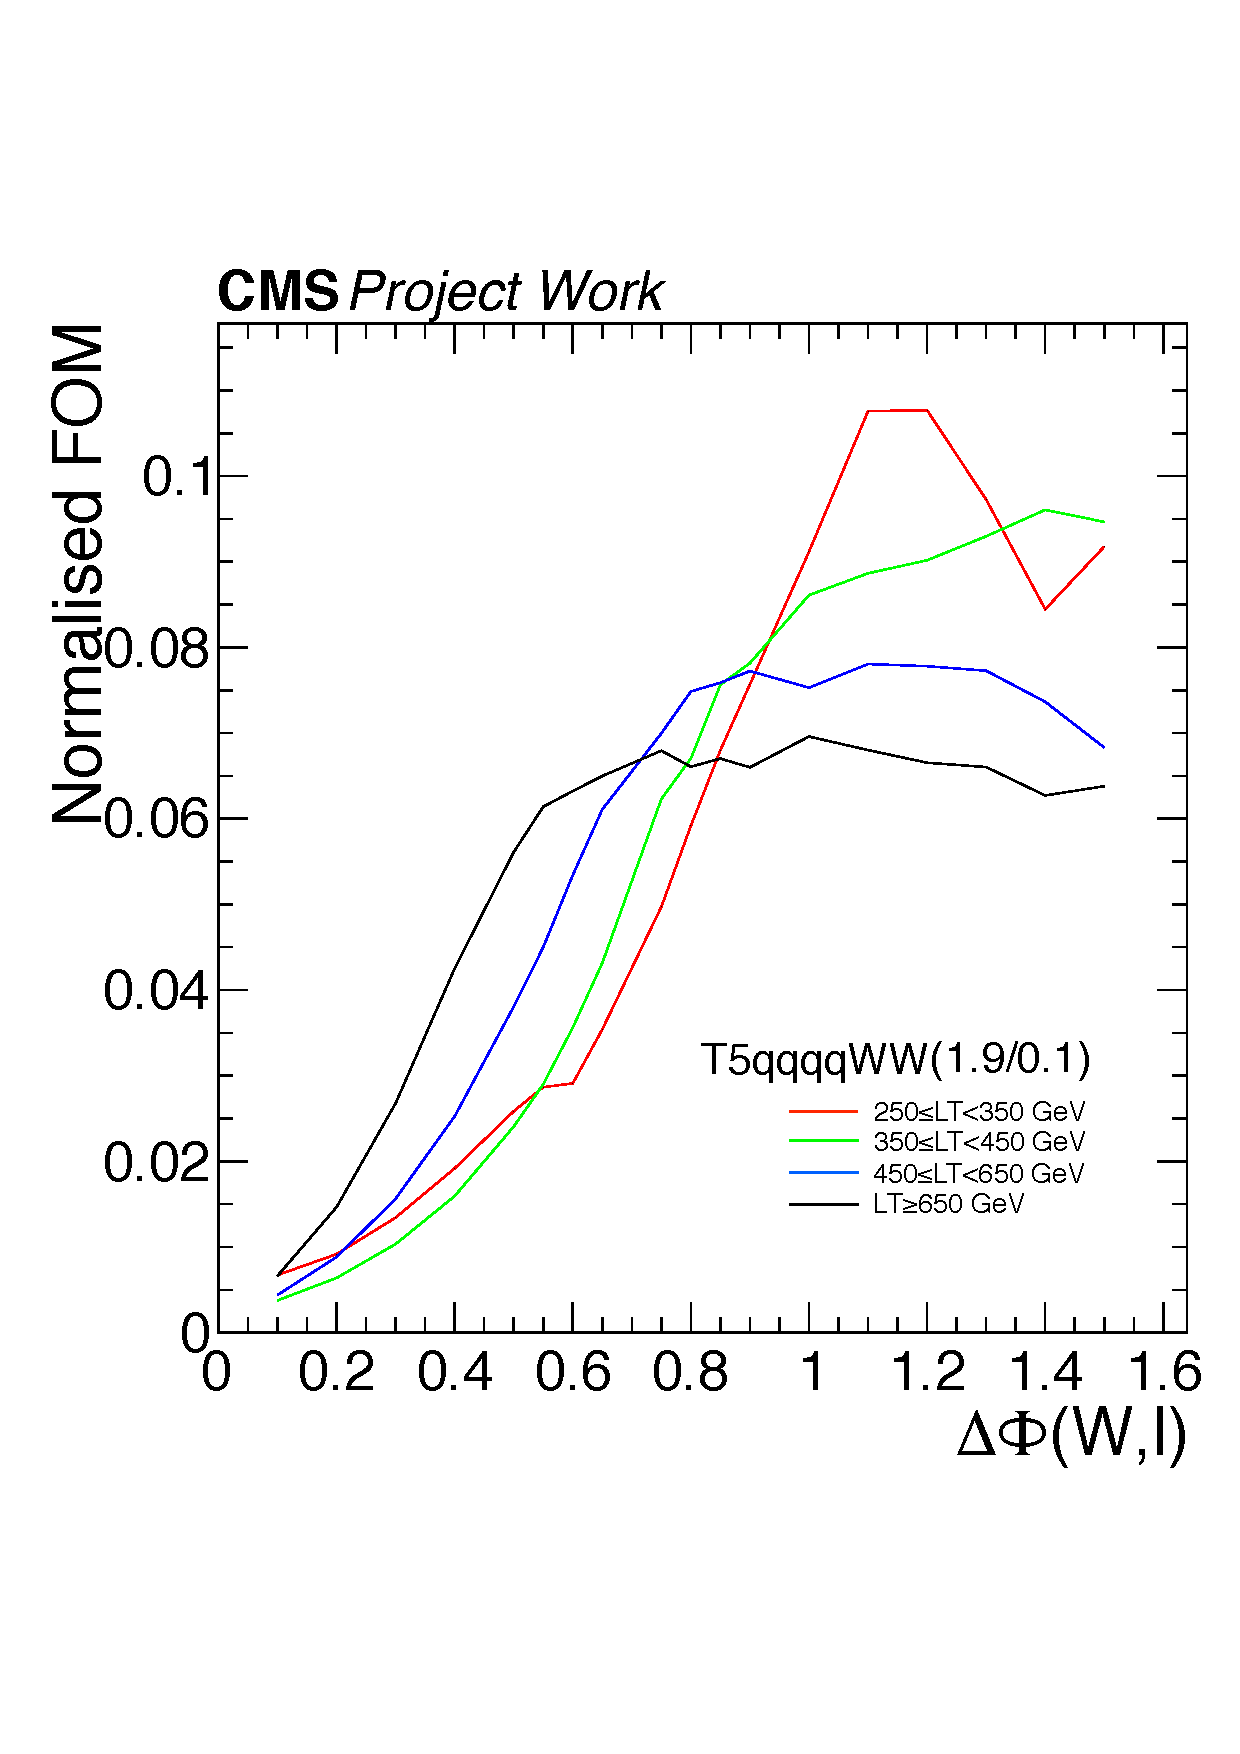
\includegraphics[width=0.45 \textwidth]{PhD_Thesis_v4/Plots/analysis/signalRegions/FOM_2.pdf}
  \caption{ \label{fig:FOM} The figure of met as a function of $\DF$ is shown for T5qqqWW(1900,100) after the baseline selection.
  }
   \end{center}
\end{figure*}
 \begin{figure*}[!h]
    \begin{center}
 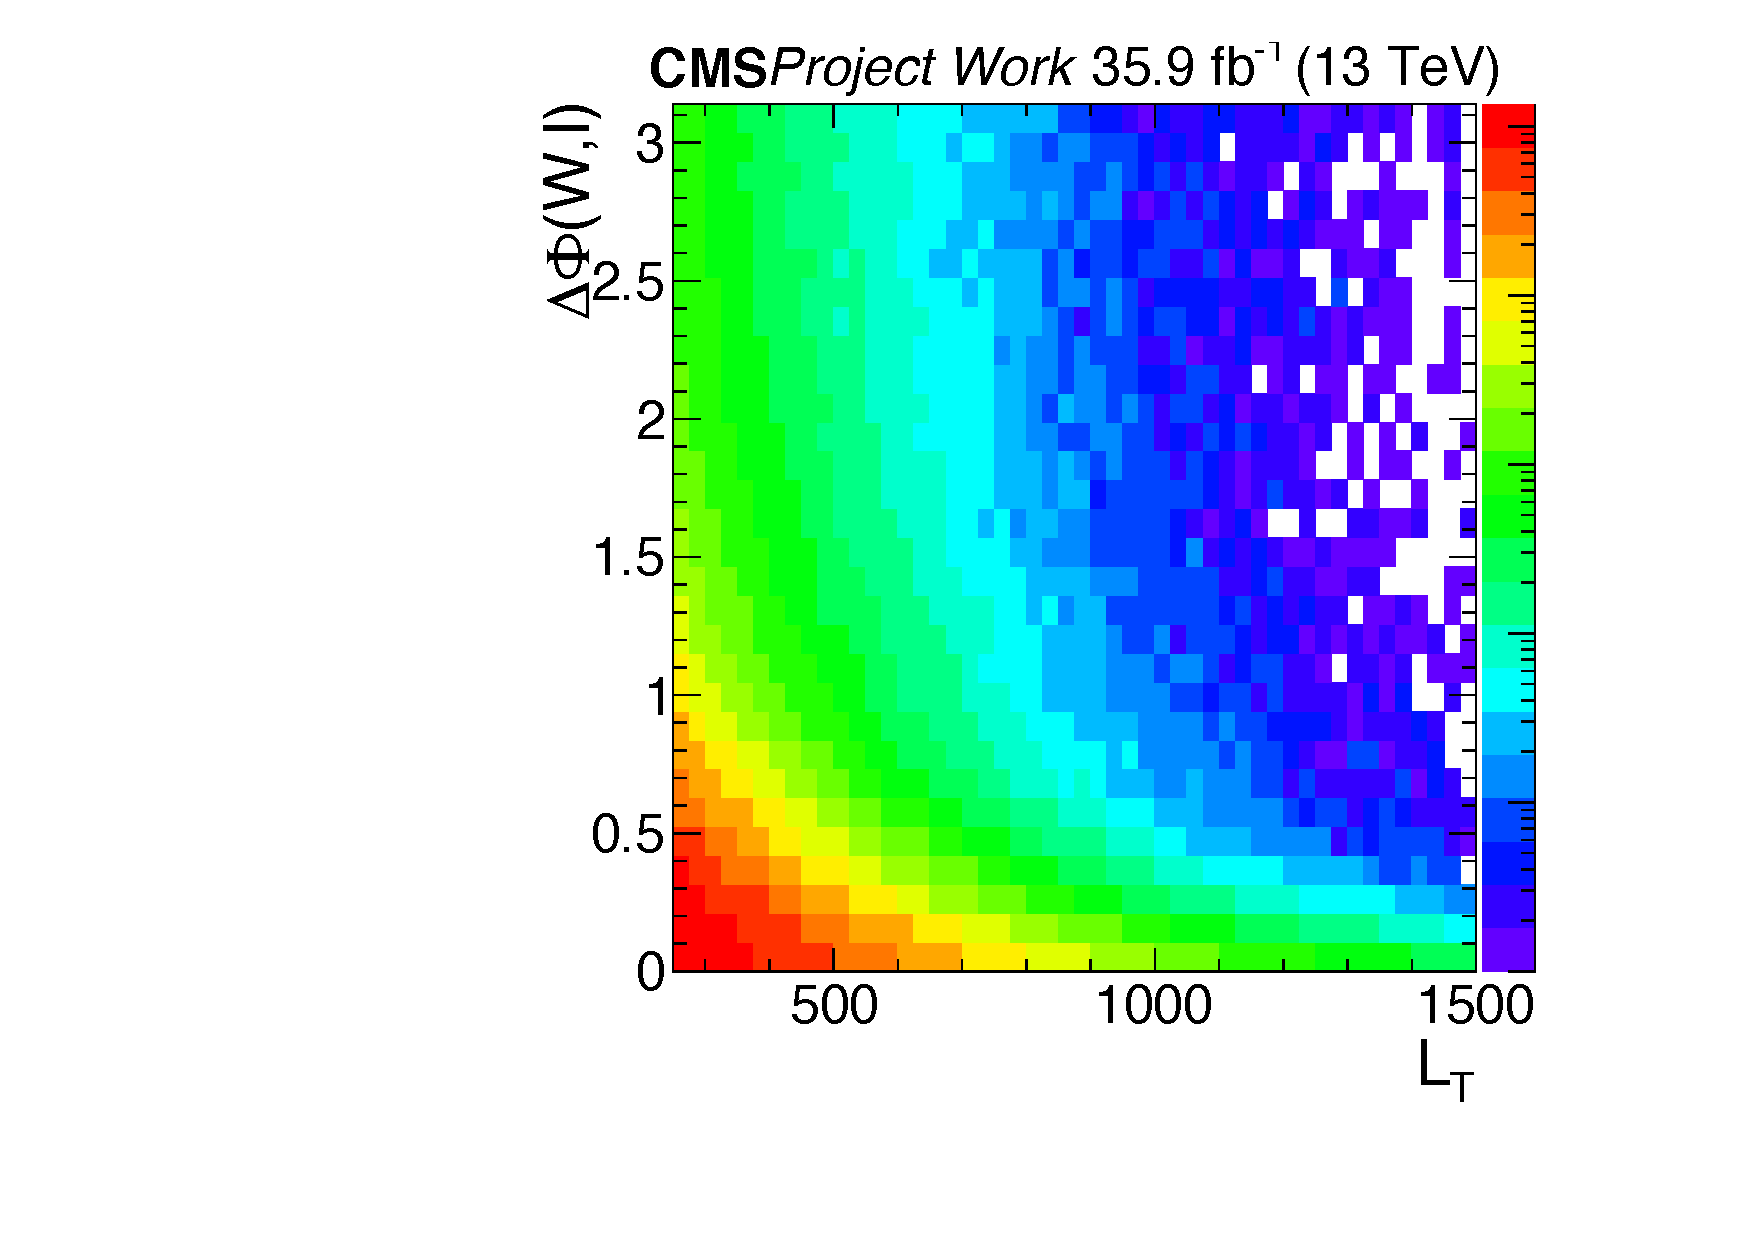
\includegraphics[width=0.45 \textwidth]{Plots/analysis/signalRegions/2D_TTWJets}\\
 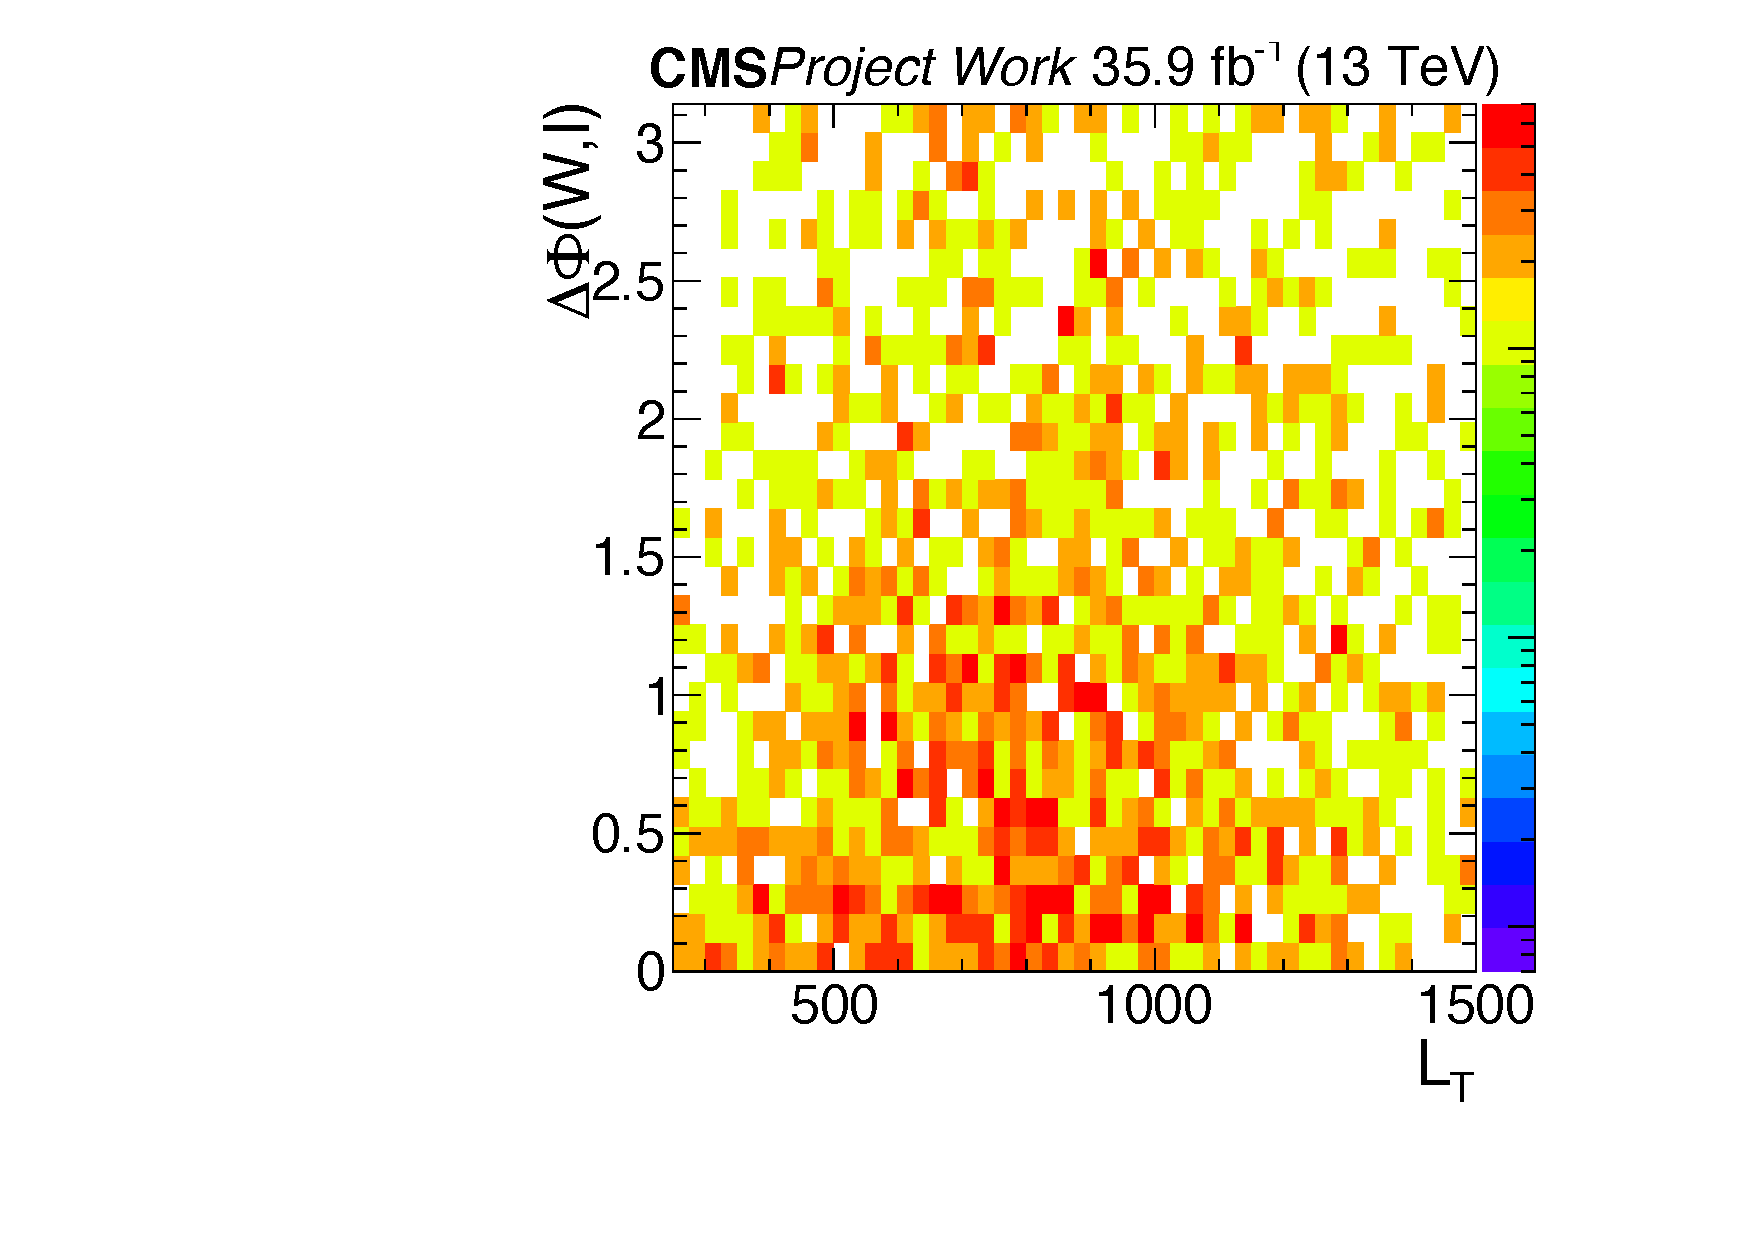
\includegraphics[width=0.45 \textwidth]{Plots/analysis/signalRegions/2D_s1900_100}
 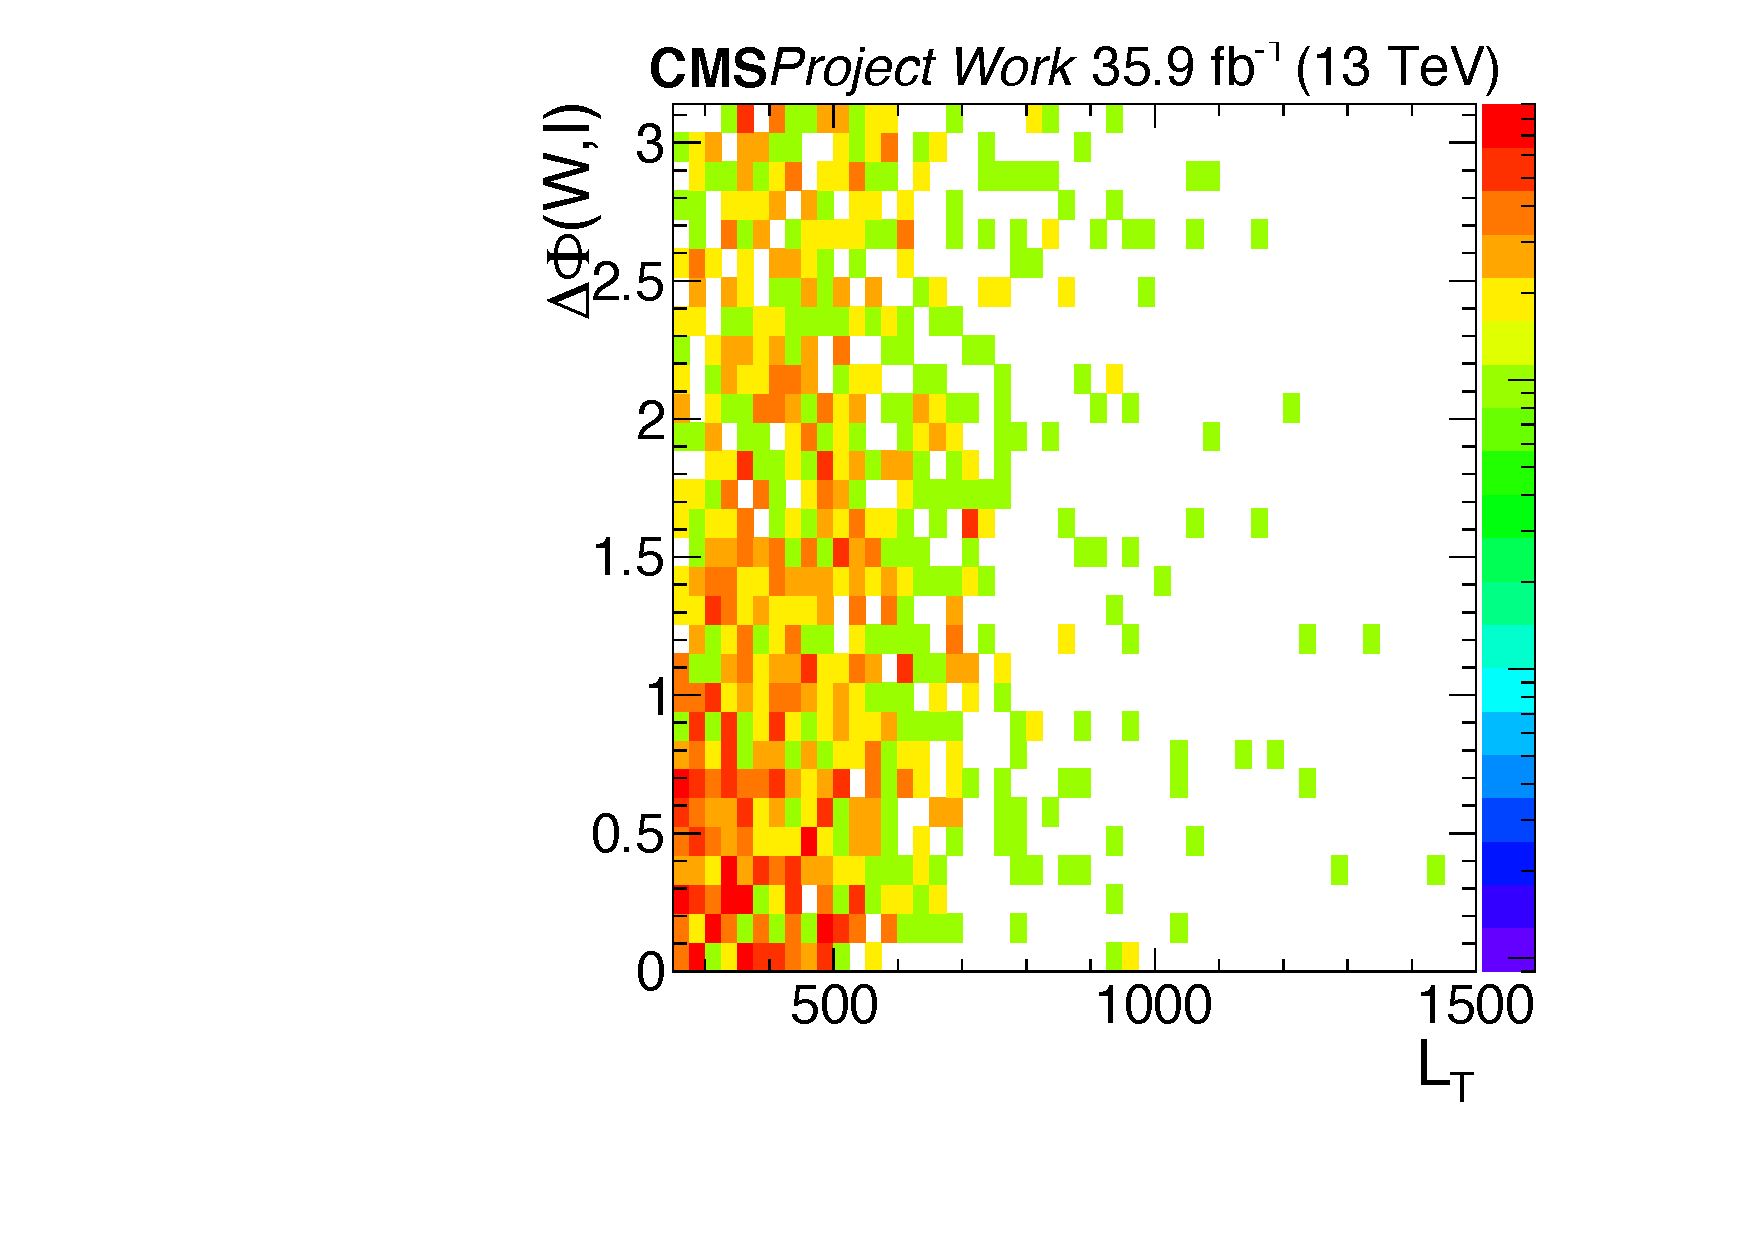
\includegraphics[width=0.45 \textwidth]{Plots/analysis/signalRegions/2D_s1500_1000}
  \caption{ \label{fig:2Ds} Two dimensional distributions of event counts for the main background samples, $\ttJets$ +$\wJets$ simulation (top), and the signal T5qqqWW(1900,100) (left) and T5qqqWW(1500,1000) in the the $\DF$ vs. $\LT$ plane after the baseline selection.
  }
   \end{center}
\end{figure*}
\textbf{Signal acceptance}\\
The yield after baseline selection for the simulated signal events is shown in Fig.~\ref{fig:signalEffs} in the gluino-neutralino mass plane for the T5qqqqWW model. The acceptance of at least one event for 35.9~fb$^{-1}$ integrated luminosity reaches up to 2250 GeV for gluino mass for the neutralinos masses below 1600 GeV. The selection efficiency, defined as the fraction of simulated signal events after the baseline requirement over the total number of simulated signal events, is presented in the same figure~(top right).
Figures~\ref{fig:signalEffs}~(bottom) show the MB~SR efficiencies. The plot on the left displays the efficiency using a constant $\DF>1$ cut. The efficiency is ranges from 50\% to 70\%. On the other hand, the right plot shows the efficiency for the $\DF$ cut taking values according to corresponding $\LT$ bin and this time the efficiency goes up to 80\%.
\begin{figure*}[!hbt]
    \begin{center}
 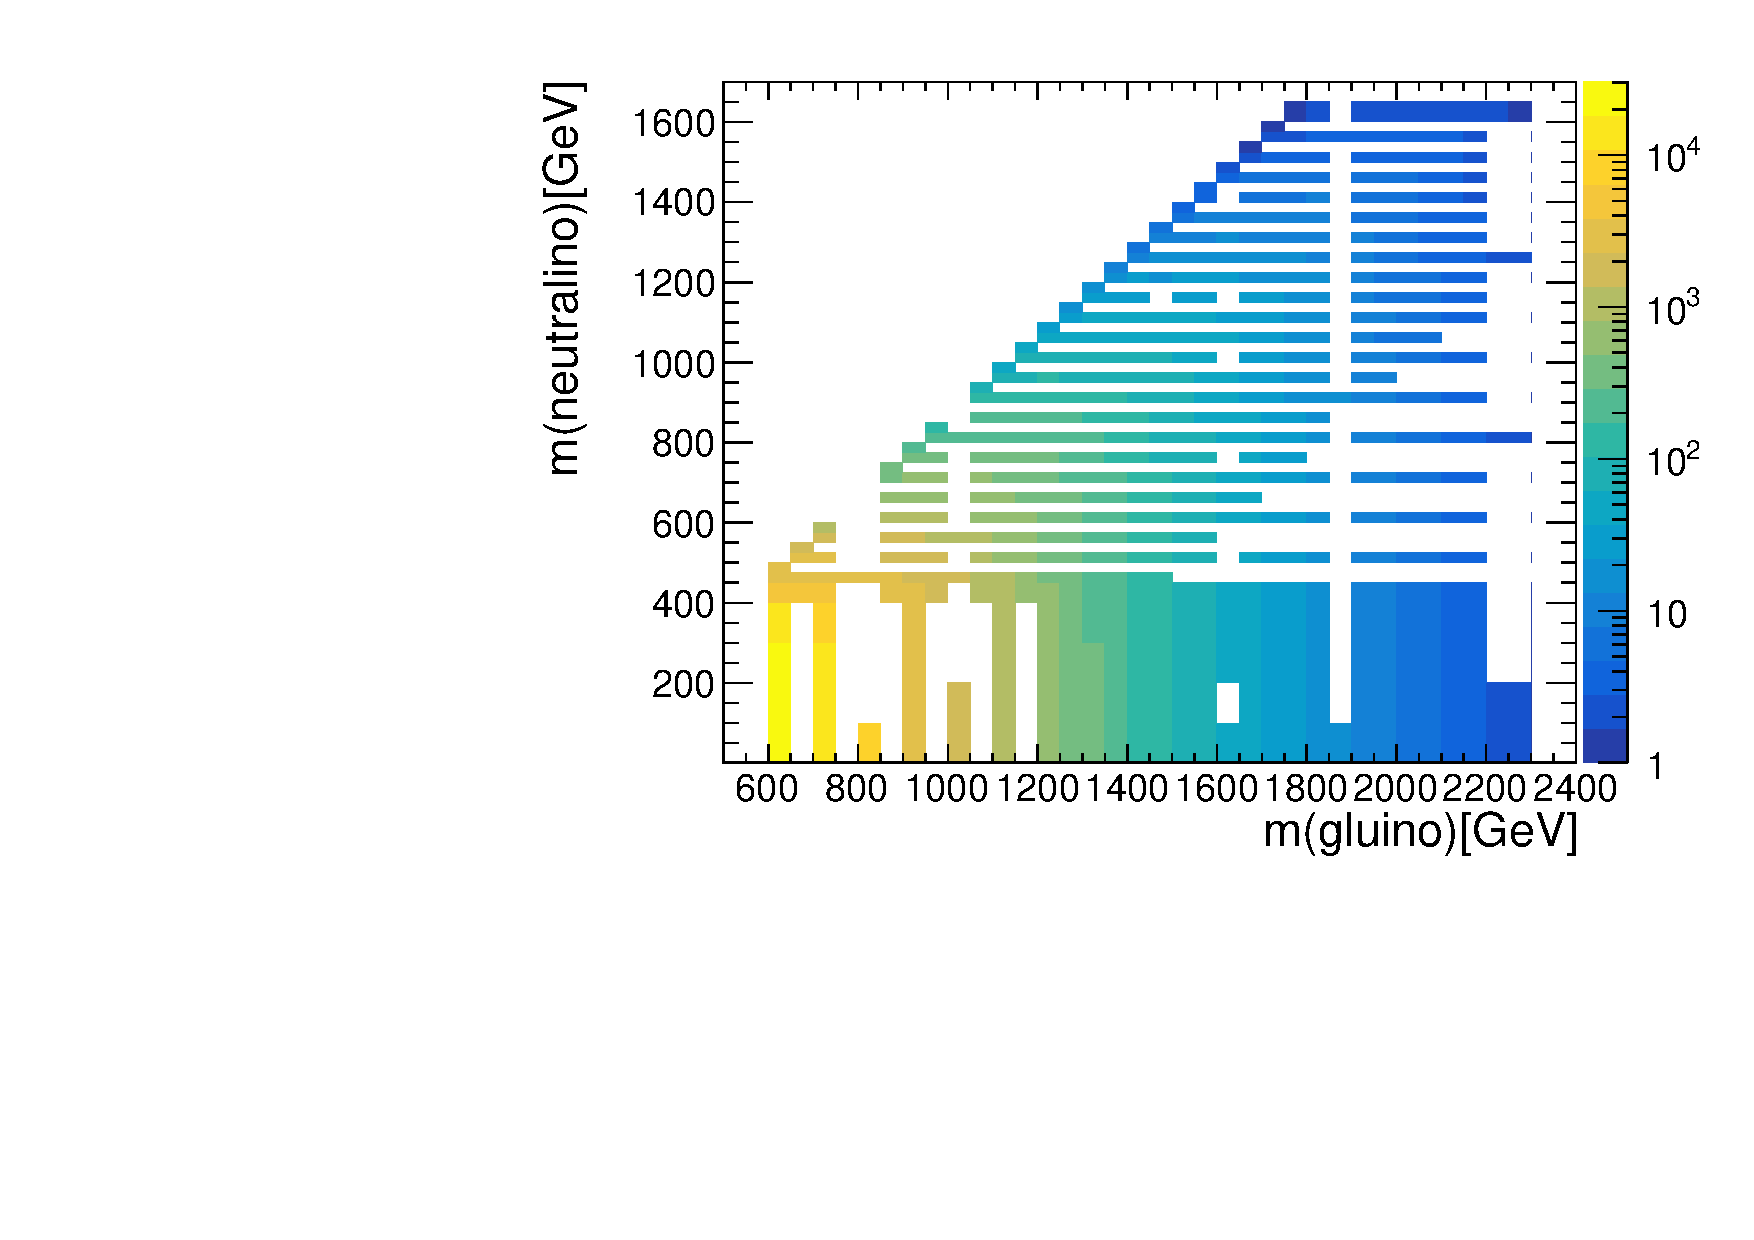
\includegraphics[width=0.45 \textwidth]{Plots/analysis/signalRegions/preselyields}
 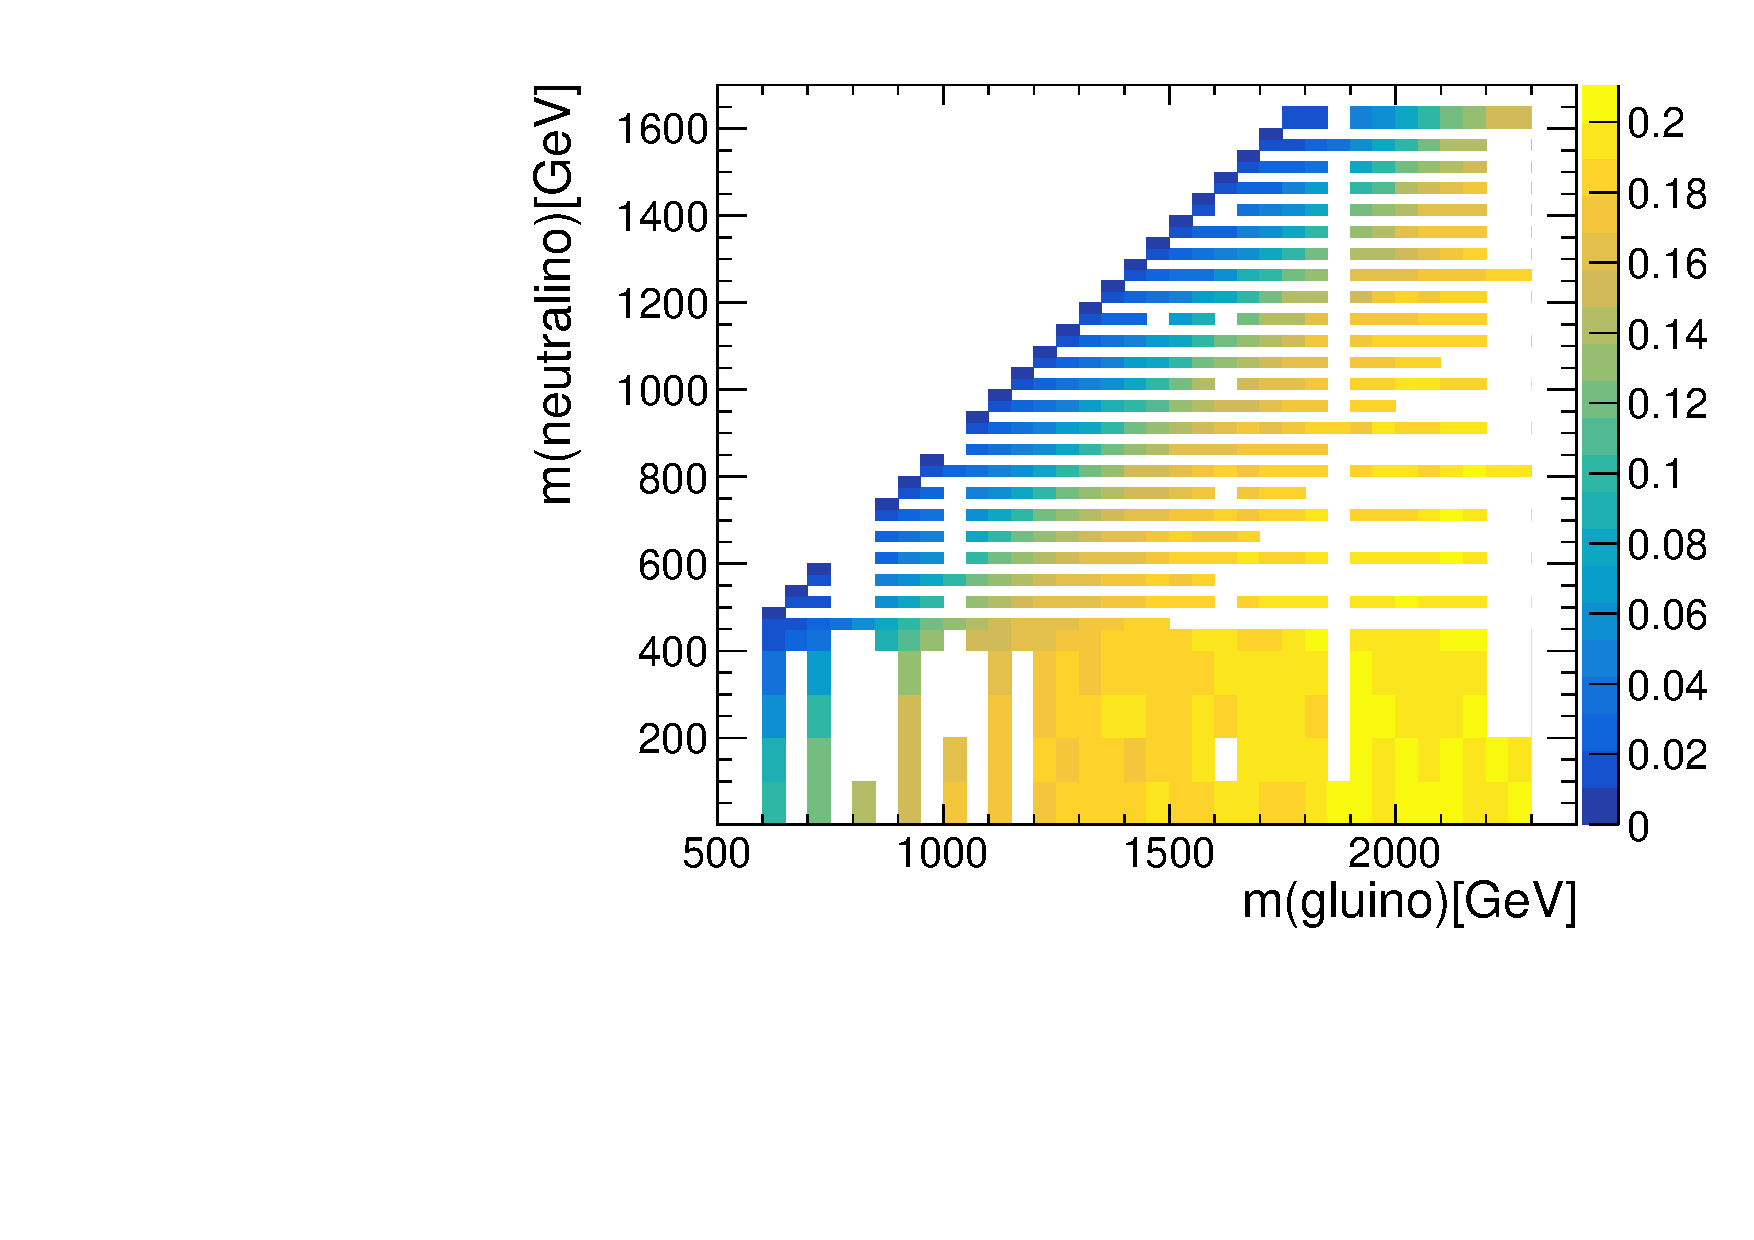
\includegraphics[width=0.4 \textwidth]{Plots/analysis/signalRegions/preselEff}\\
 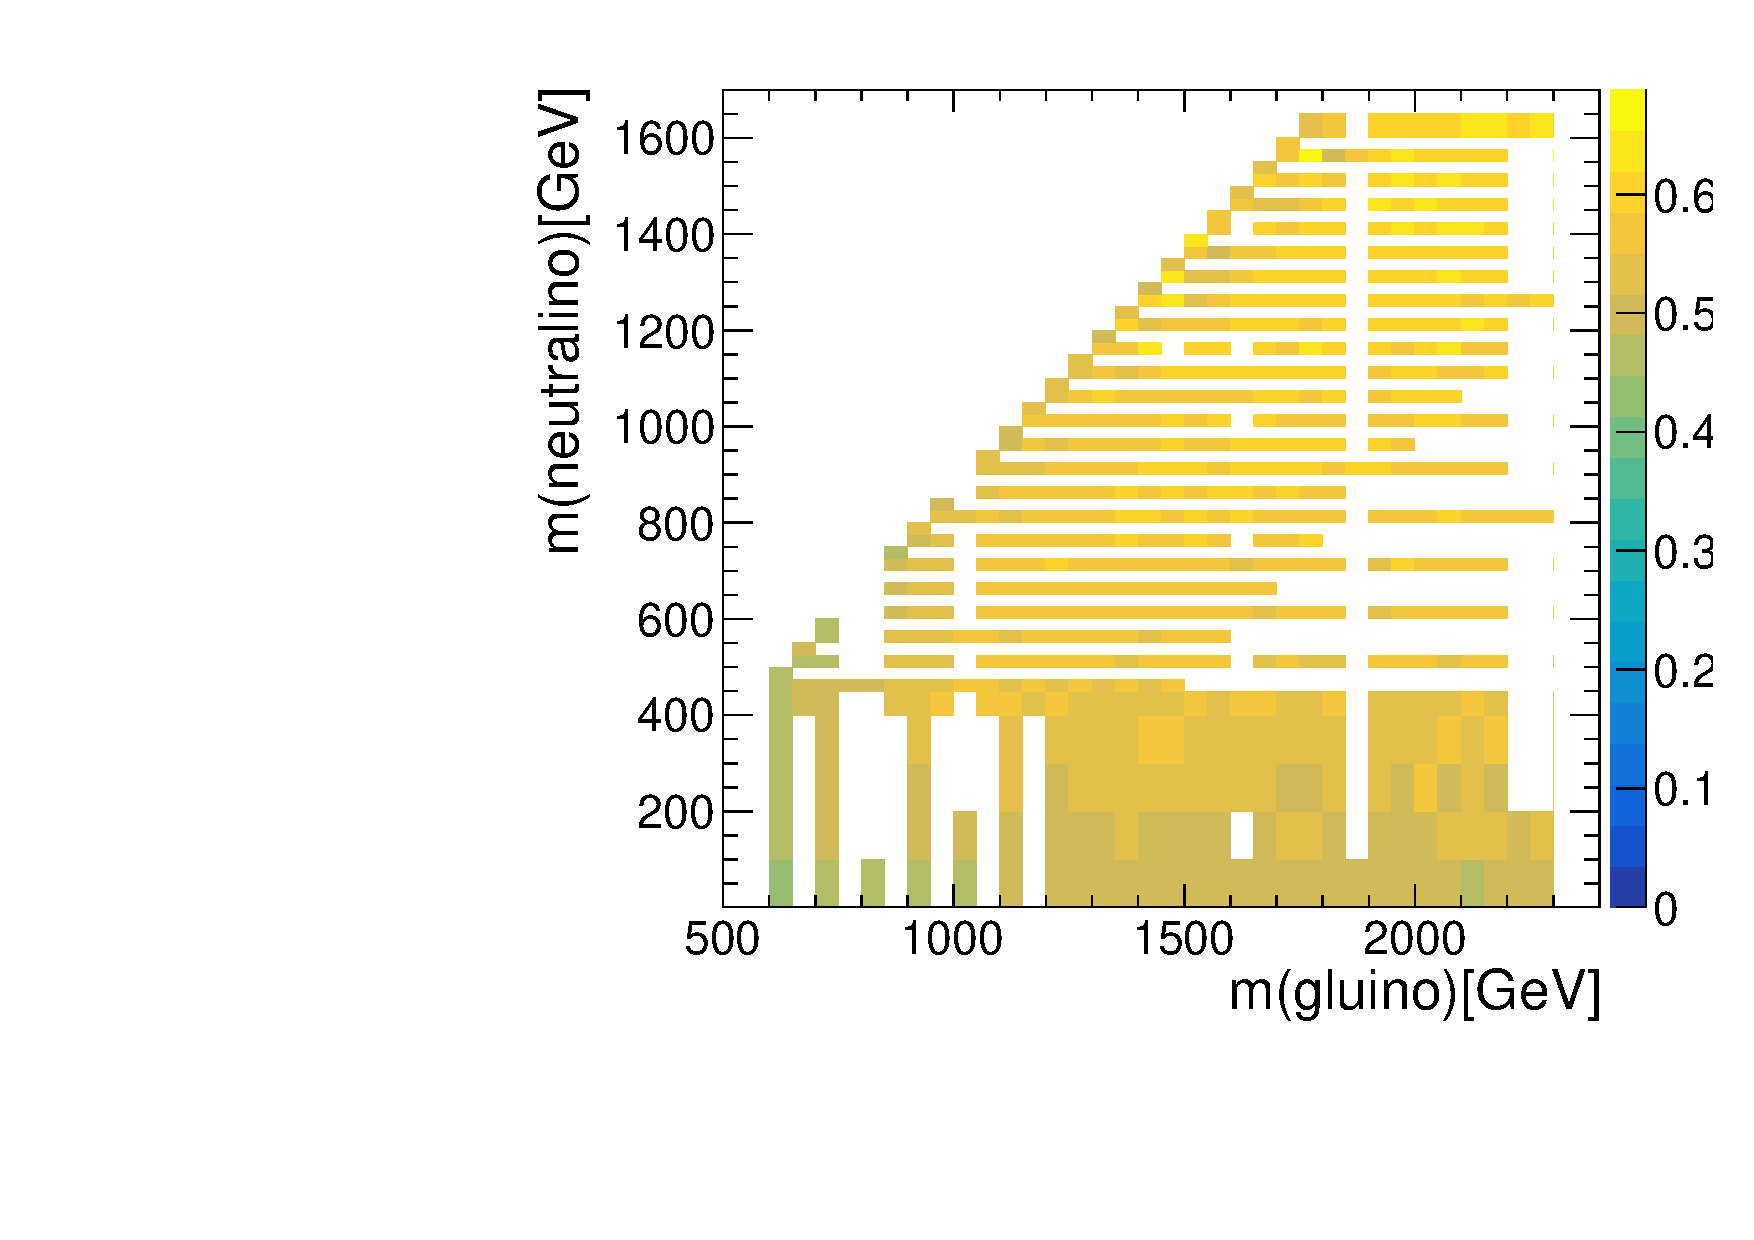
\includegraphics[width=0.4 \textwidth]{Plots/analysis/signalRegions/DF_Eff}
  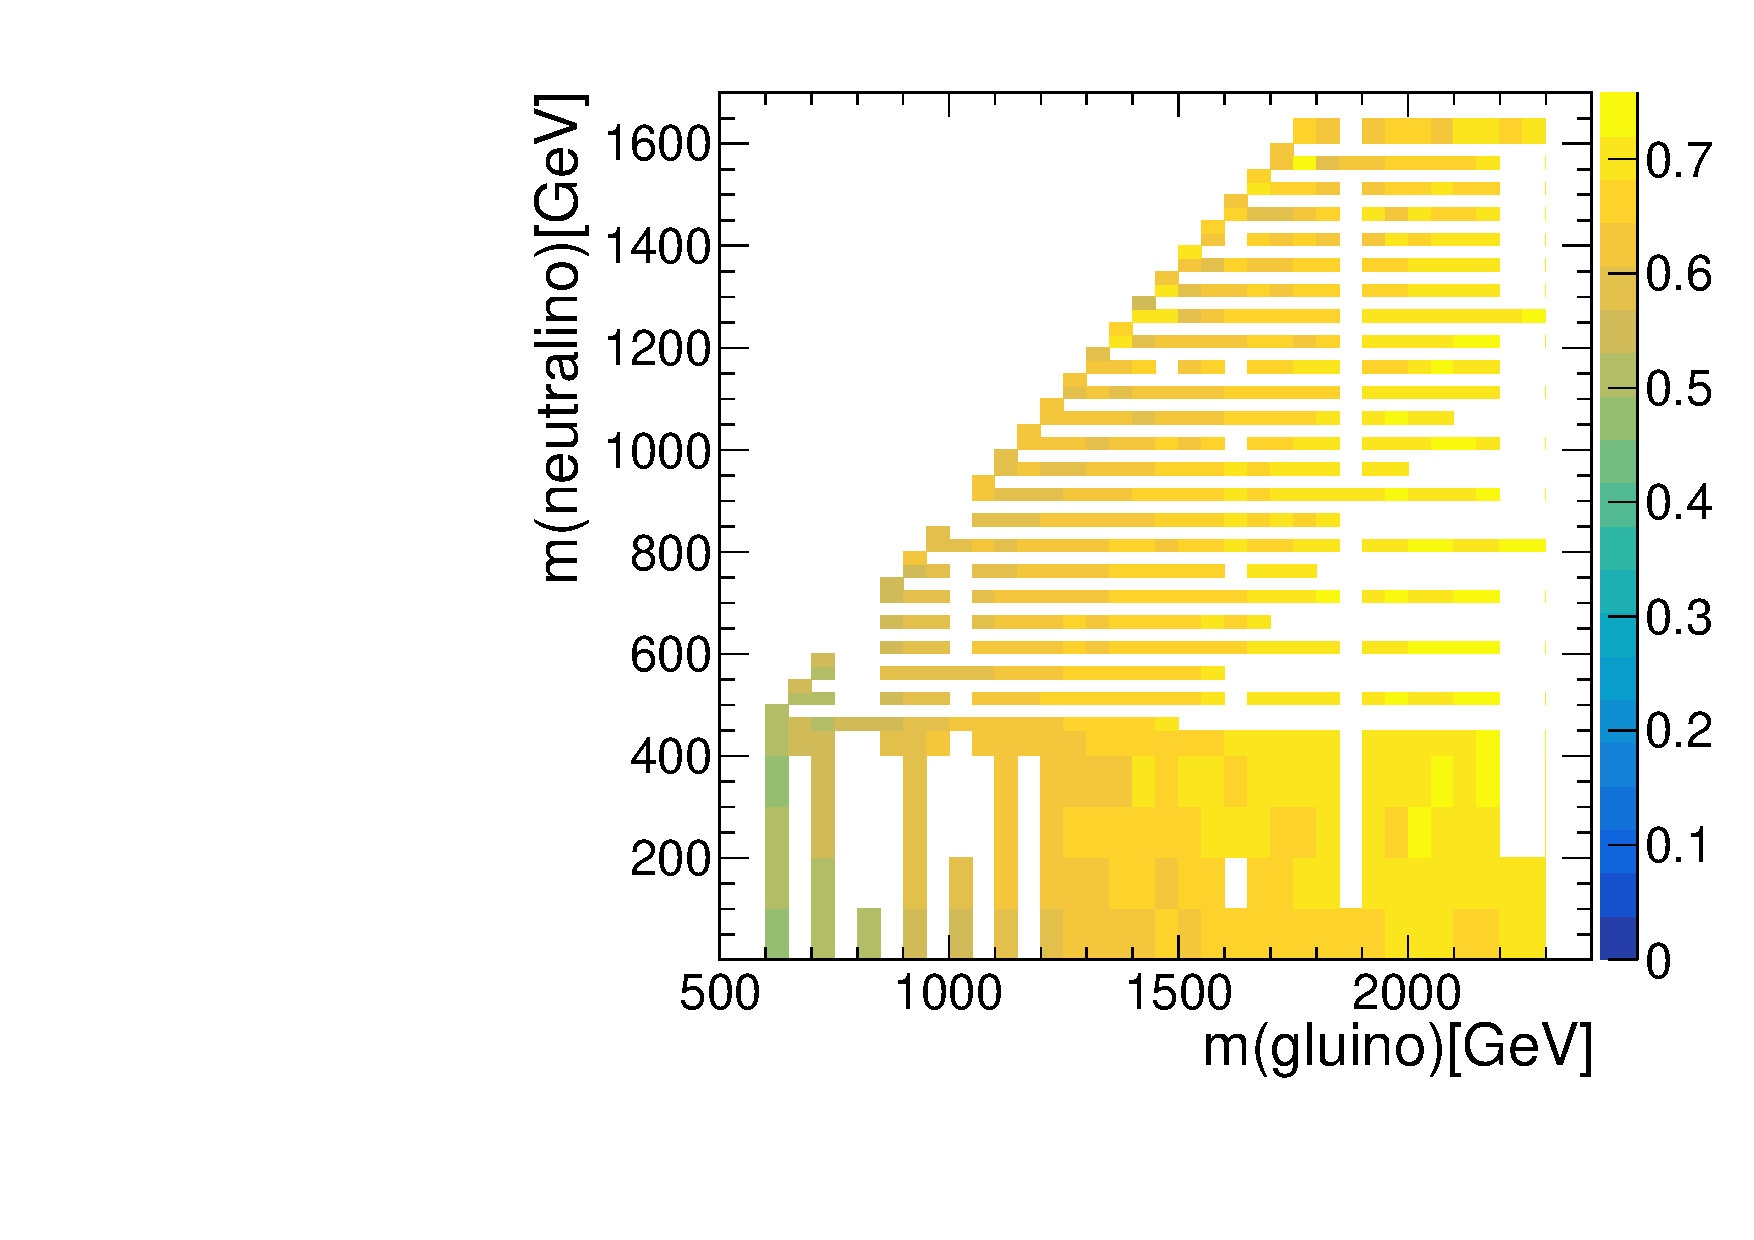
\includegraphics[width=0.4 \textwidth]{Plots/analysis/signalRegions/DF_var_Eff}
  \caption{ \label{fig:signalEffs} The distributions on top represent T5qqqqWW signal counts~(left) and selection efficiency (right) after the baseline requirements in the gluino-neutralino plane. The distributions at the bottom show the efficiency of signal region selection with respect to the baseline selection; $\DF>1$~(left) and $\DF>x$~(right) where x is the threshold according to $\LT$ bin.  
  }
   \end{center}
\end{figure*}

 \begin{figure*}[!hbt]
    \begin{center}
 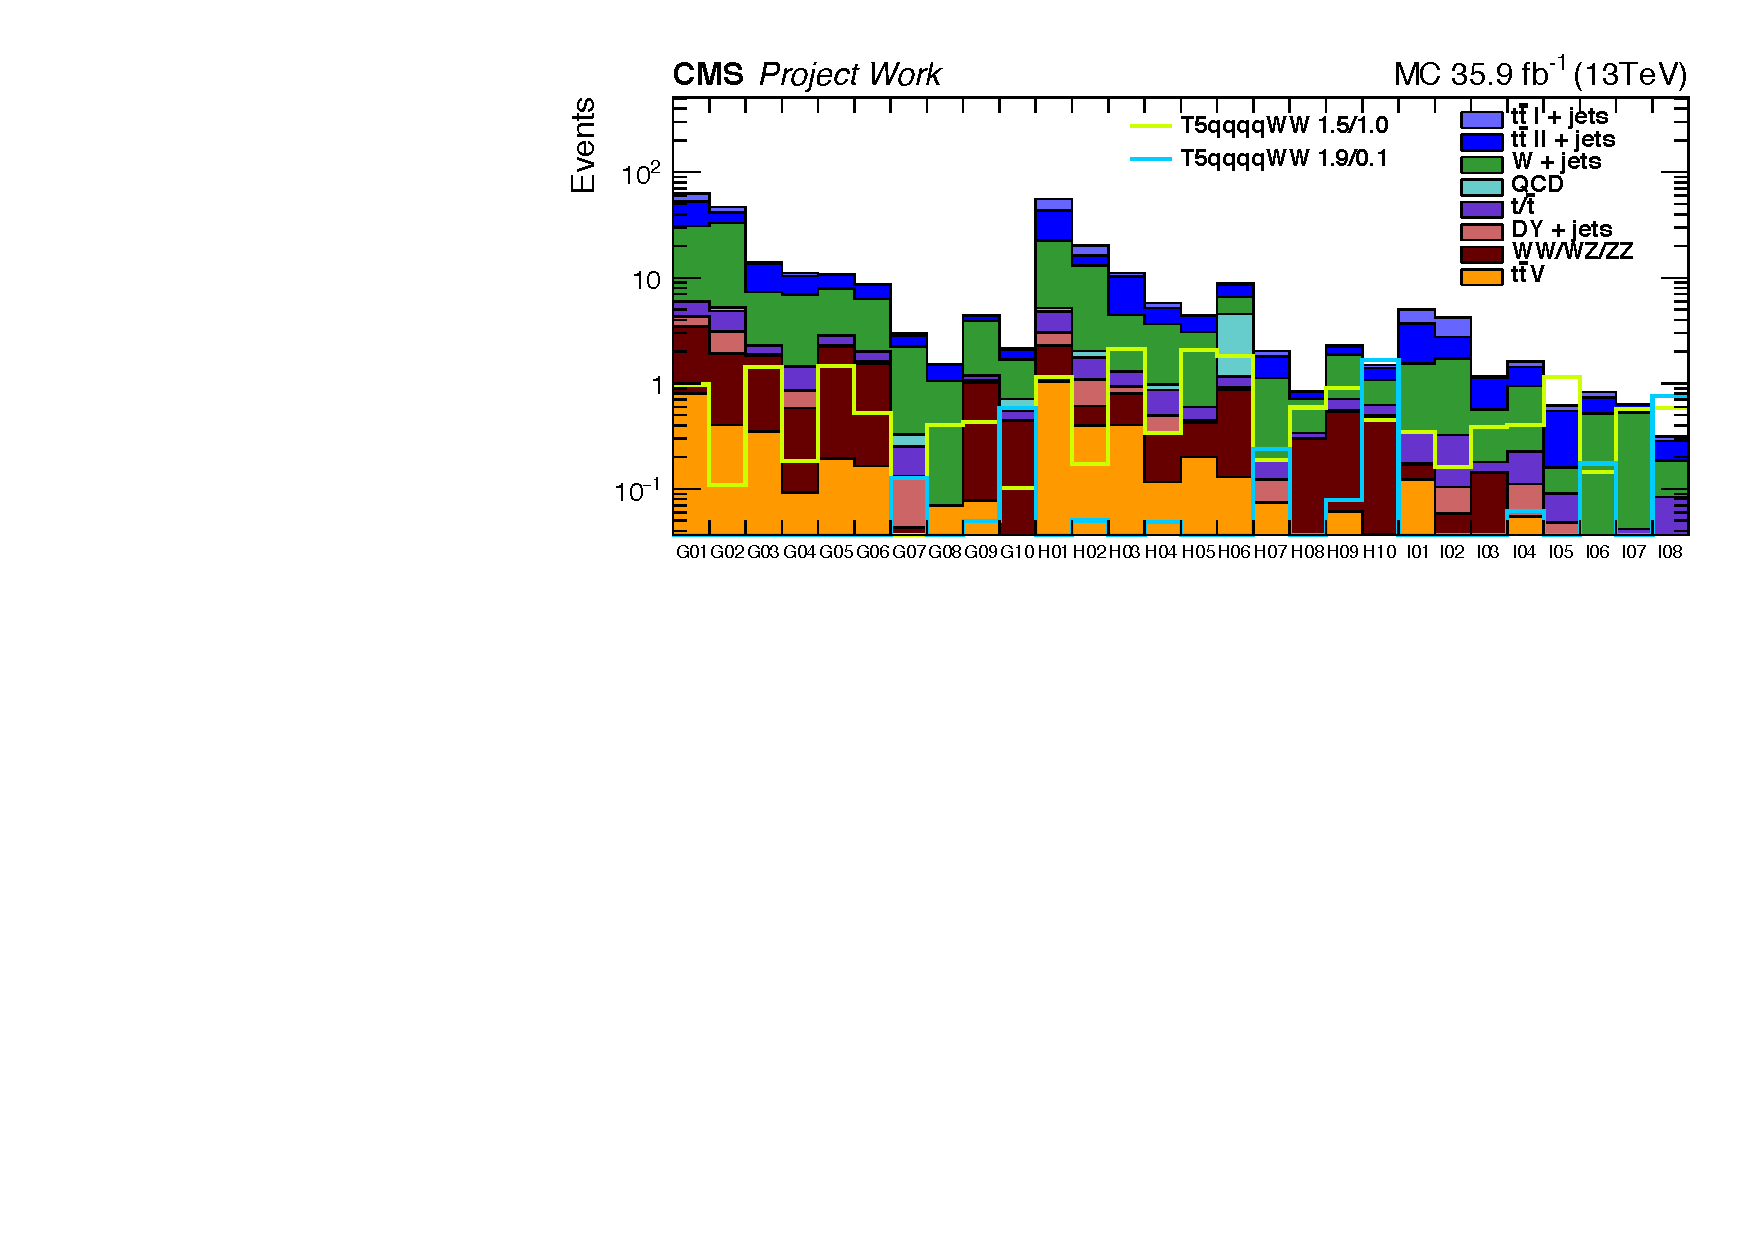
\includegraphics[width=0.95 \textwidth]{Plots/analysis/signalRegions/MC__mu__SR}\\
   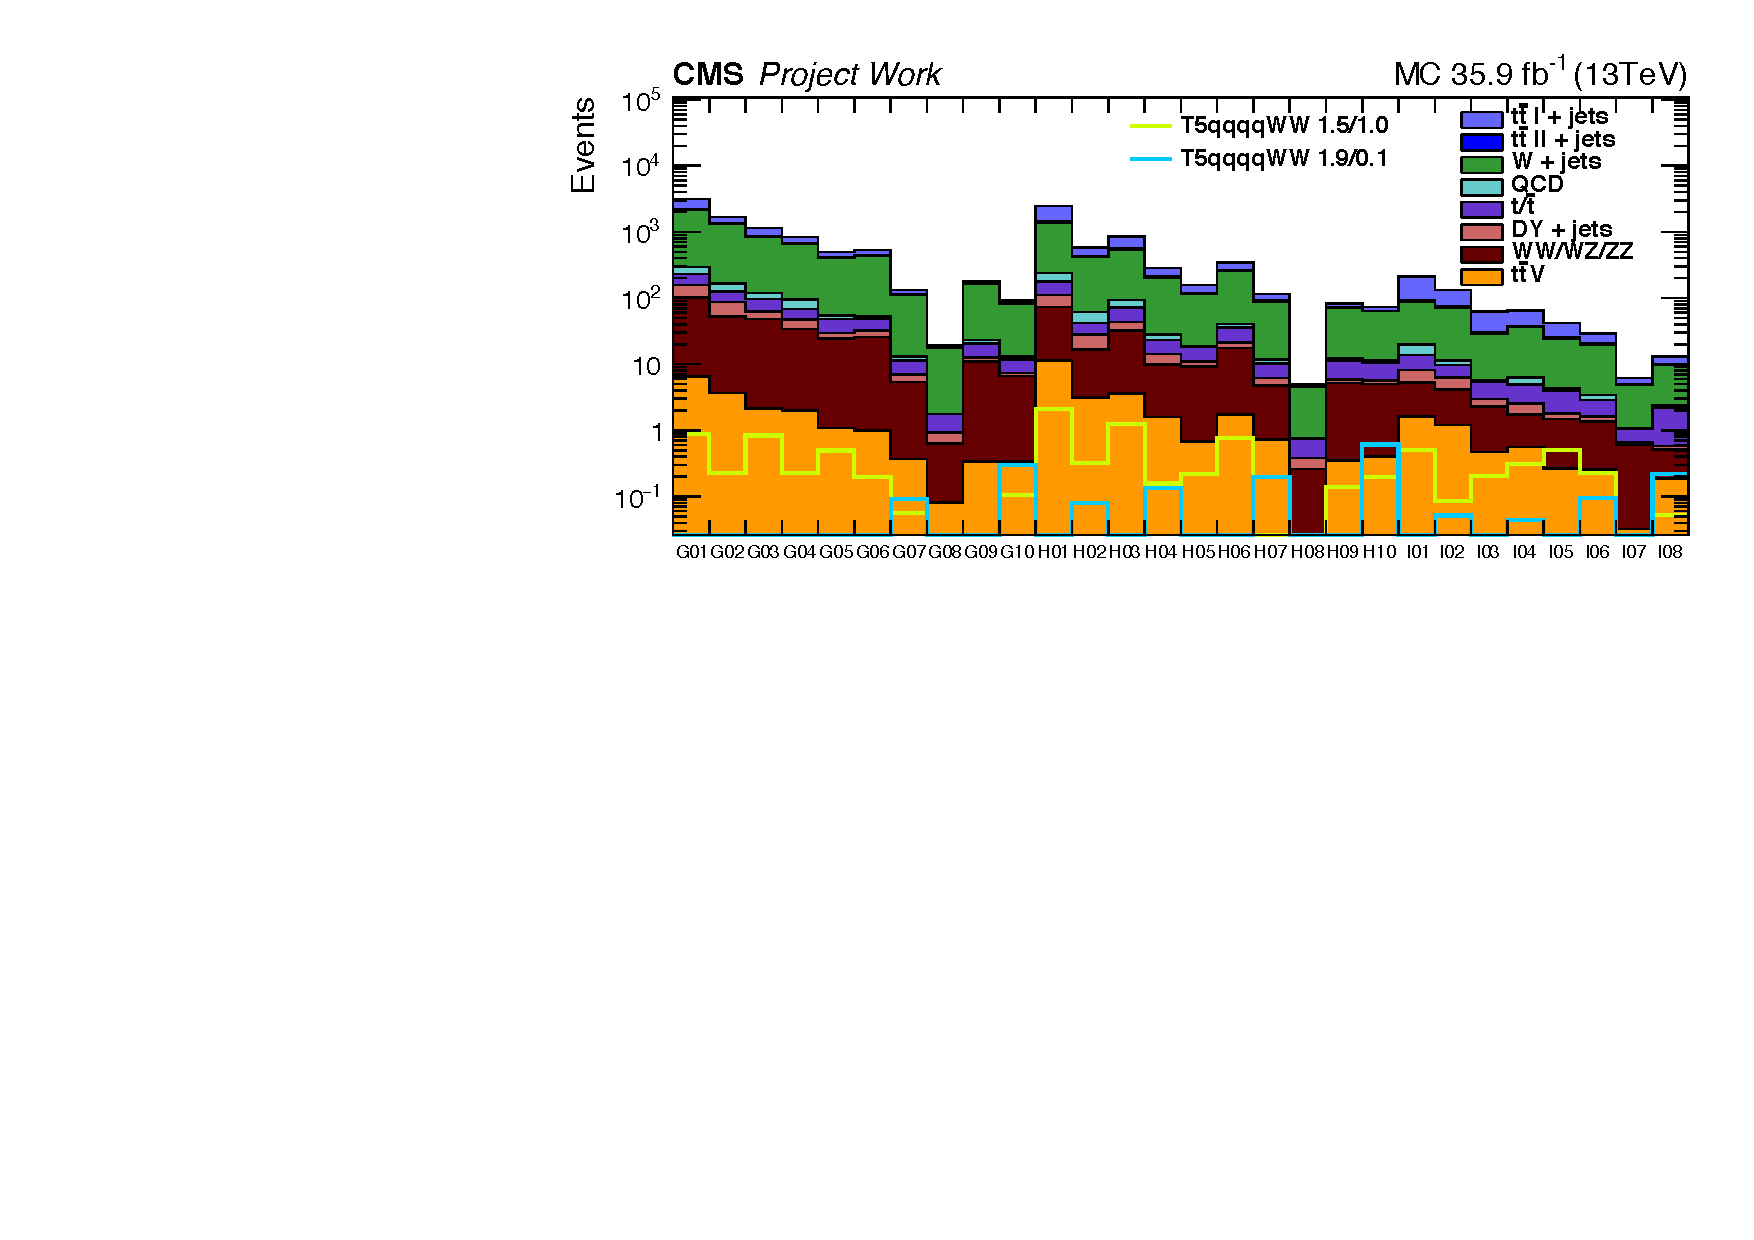
\includegraphics[width=0.95 \textwidth]{Plots/analysis/signalRegions/MC__mu__CR}
  \caption{ \label{fig:MCcounts_mu} Simulated single muon event yields for the background processes are shown as color filled stacked histograms for all 28 search bins. The two signal benchmark models are overlayed and shown by line histograms. The upper plot shows the high $\DF$ regions (SR) while the lower plot shows the low $\DF$ regions (CR).
  }
   \end{center}
\end{figure*}

 \begin{figure*}[!hbt]
    \begin{center}
 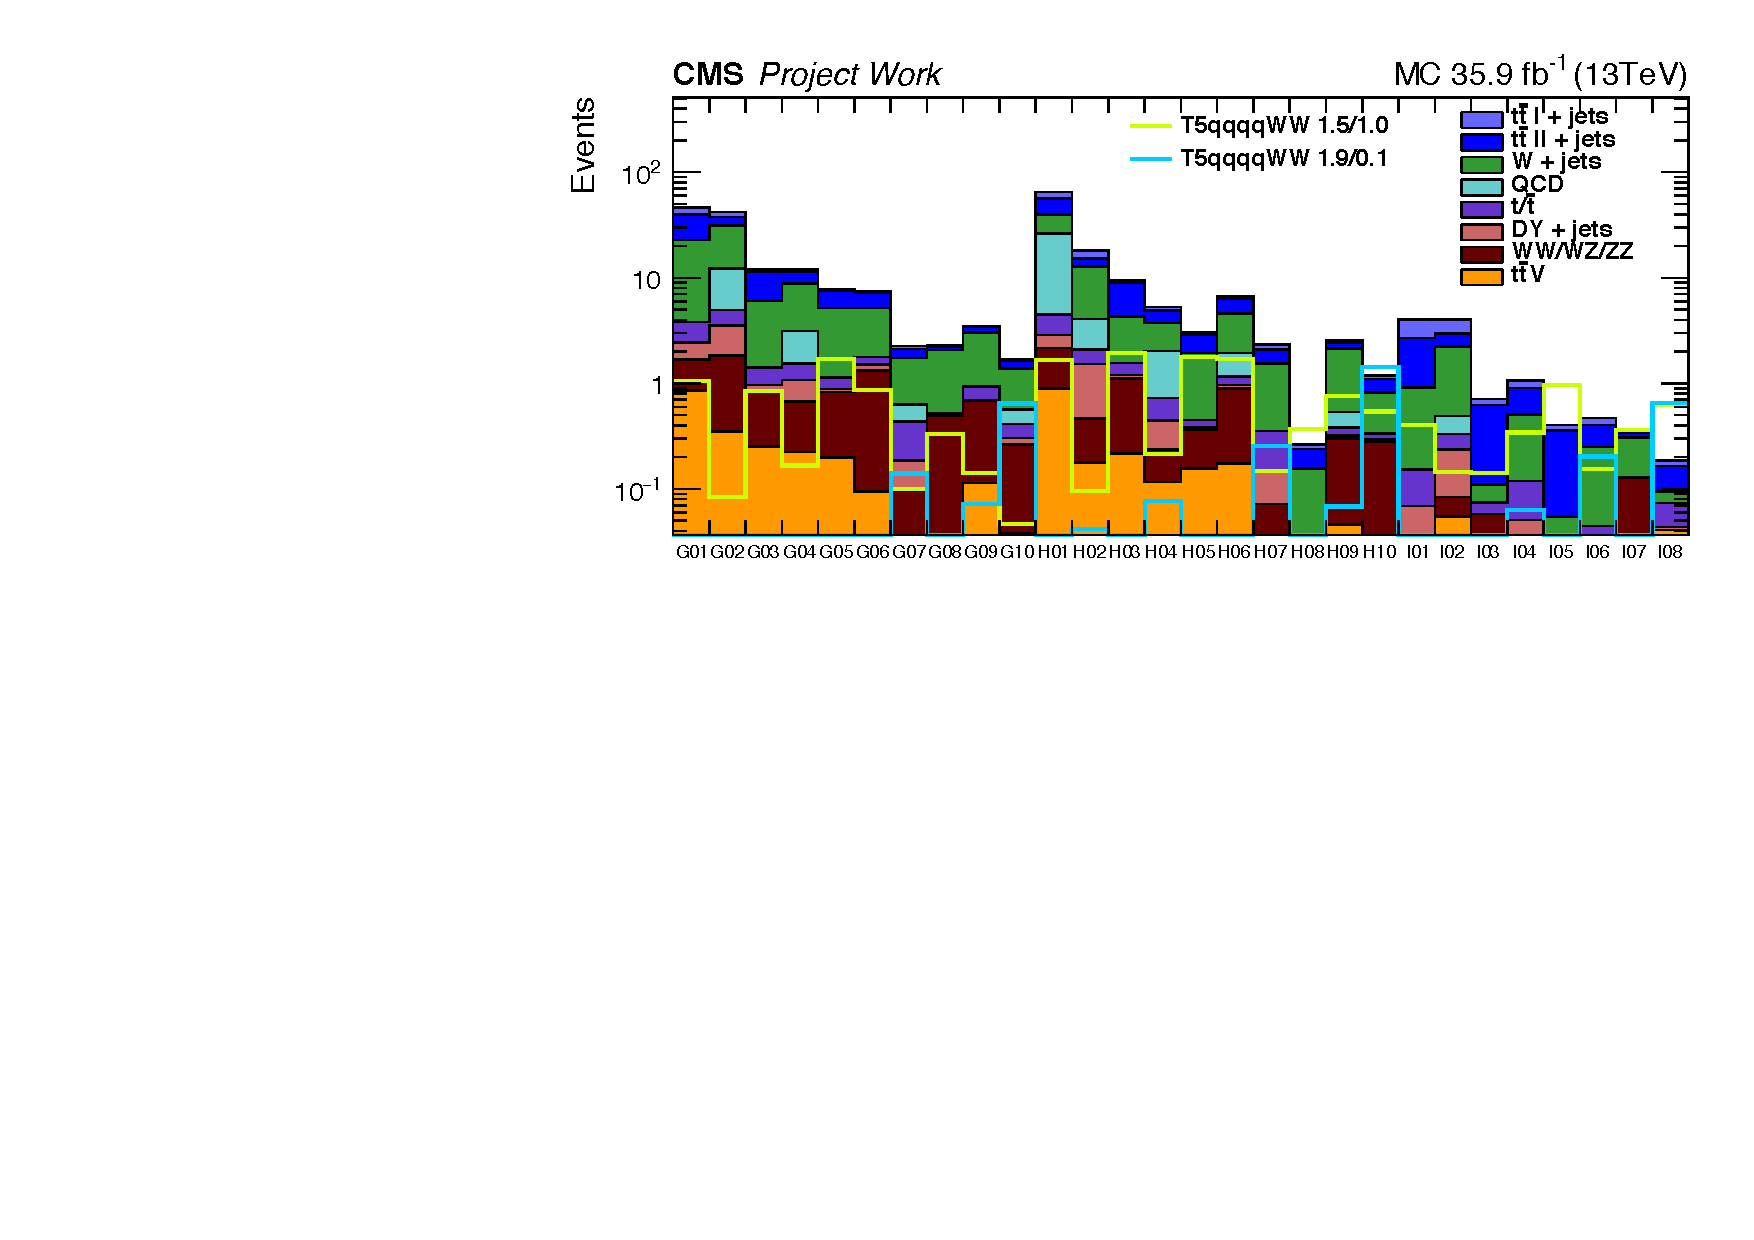
\includegraphics[width=0.95 \textwidth]{Plots/analysis/signalRegions/MC__ele__SR}\\
   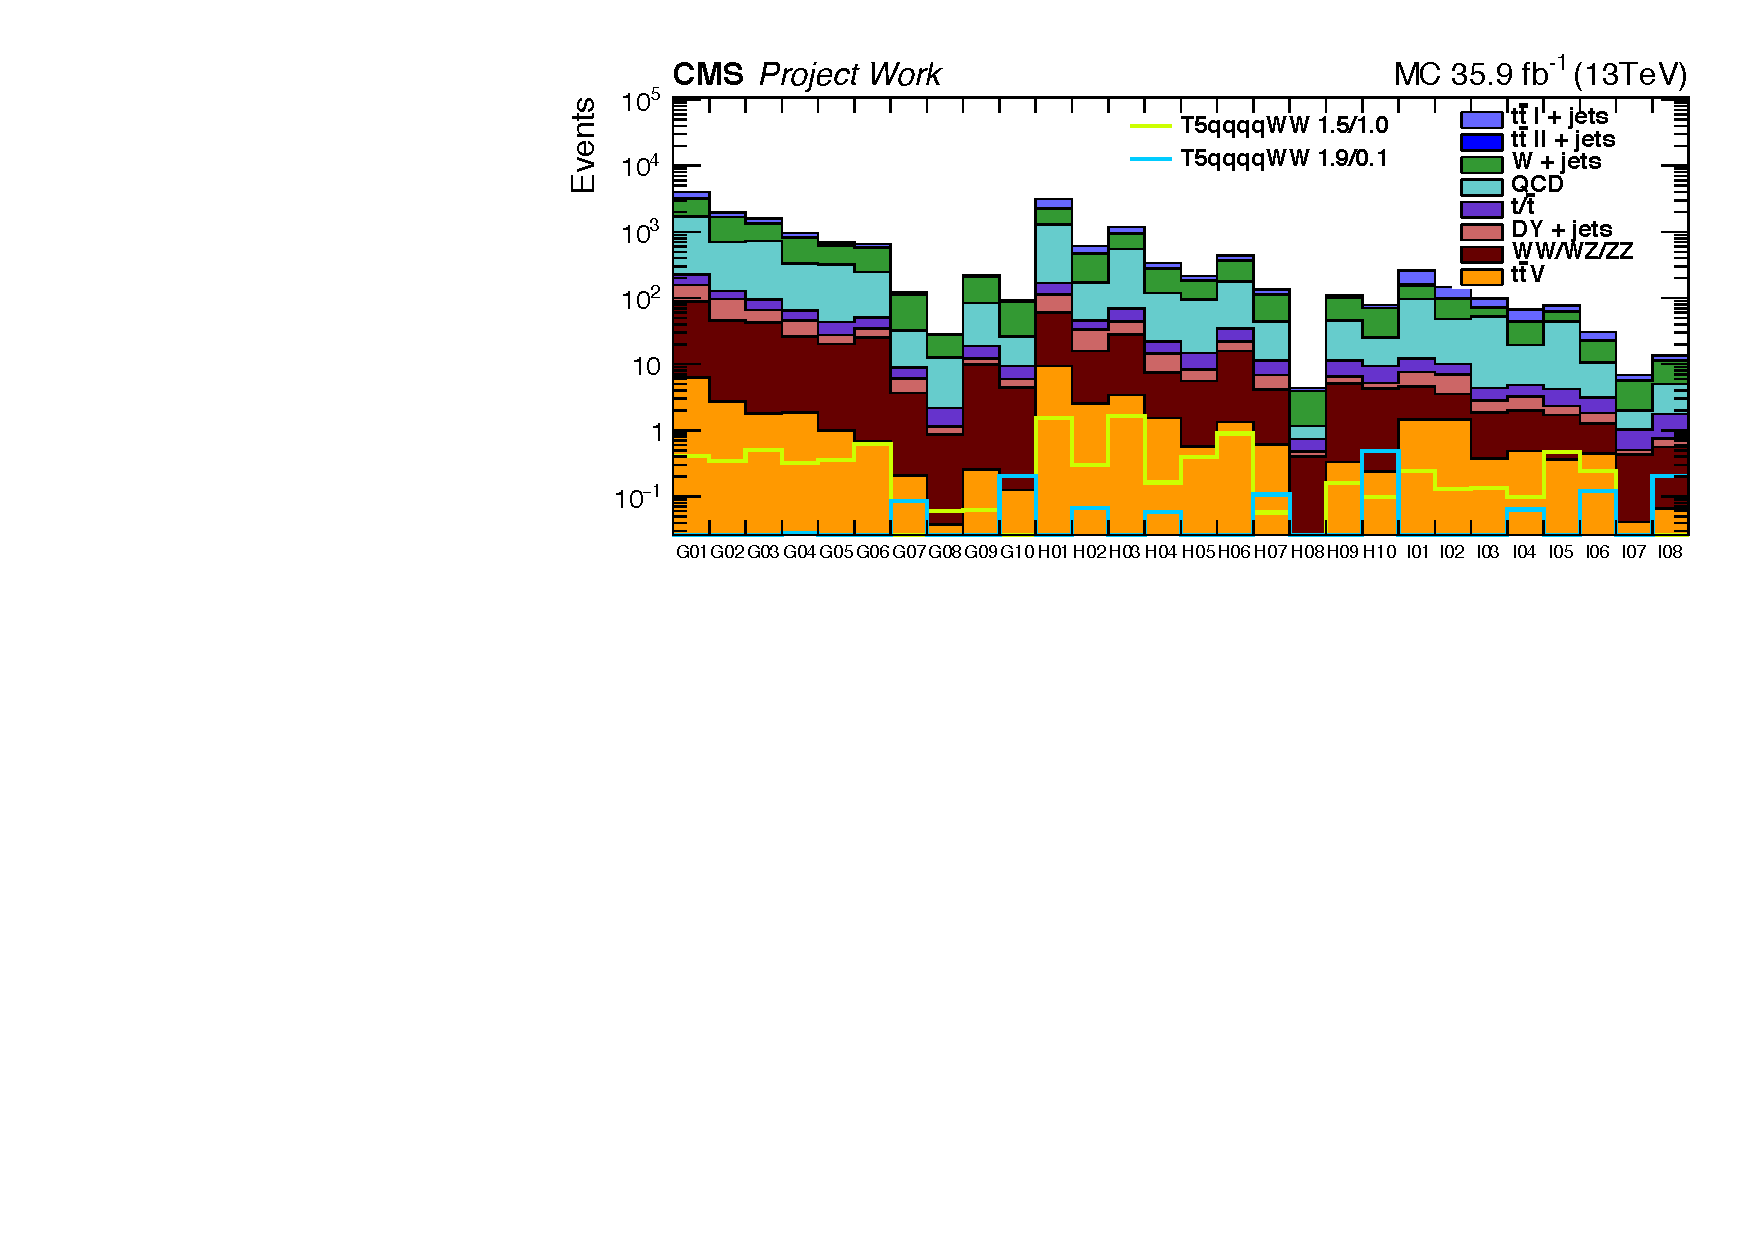
\includegraphics[width=0.95 \textwidth]{Plots/analysis/signalRegions/MC__ele__CR}
  \caption{ \label{fig:MCcounts_ele} Simulated single electron event yields for the background processes are shown as color filled stacked histograms for all 28 search bins. The two signal benchmark models are overlayed and shown by line histograms. The upper plot shows the high $\DF$ regions (SR) while the lower plot shows the low $\DF$ regions (CR).
  }
   \end{center}
\end{figure*}
\subsection{Aggregate regions}
\label{sec:aggrSR}
In order to facilitate future reinterpretations, aggregate signal regions are defined in this section. The goal of the aggregate signal regions is, to have a lower number of bins, while keeping sensitivity at an acceptable level.\\
To find optimal aggregate signal regions, 3 signal benchmark points have been used. The signal point with gluino mass 1800 GeV and neutralino mass 100 GeV is used to represent the compressed region.
For the bulk region two lower gluino mass points(1600,1300 GeV) has been used only for defining the aggregated signal regions.\\
First, an attempt is made to merge adjacent bins. 
Second, the expected exclusion is evaluated individually per bin. The result is shown in Fig.~\ref{fig:rvalues} as a function of the excluded signal strength modifier r. Last, a choice is made. Bins at high $\njet$, high $\HT$, and/or high $\LT$ are selected to form the aggregate regions and they are summarized in Tab.~\ref{tab:Aggrsim_results}.
%The expected limit on r is X while the expected limit on r for the full set of SR is Y.
%Then the r-value for these inclusive version of existing bins have been calculated, Fig.~\ref{fig:rvalues} shows r-values for each inclusive search bin.
%All of the bins shown in the figure actually overlapping and inclusive in $\HT$,$\LT$ and $\njet$.  A few bins with the lowest r-value have been chosen.\\
%Naturally, bins at high $\njet$, high $\HT$, and/or high $\LT$ are more
%sensitive to the signal. In the end, 6 inclusive bins have been defined to form the aggregate signal regions. The resulting 6 bins of the aggregated signal region are presented in Tab.~\ref{tab:Aggrsim_results}.
\begin{figure}[!h]
\begin{center}
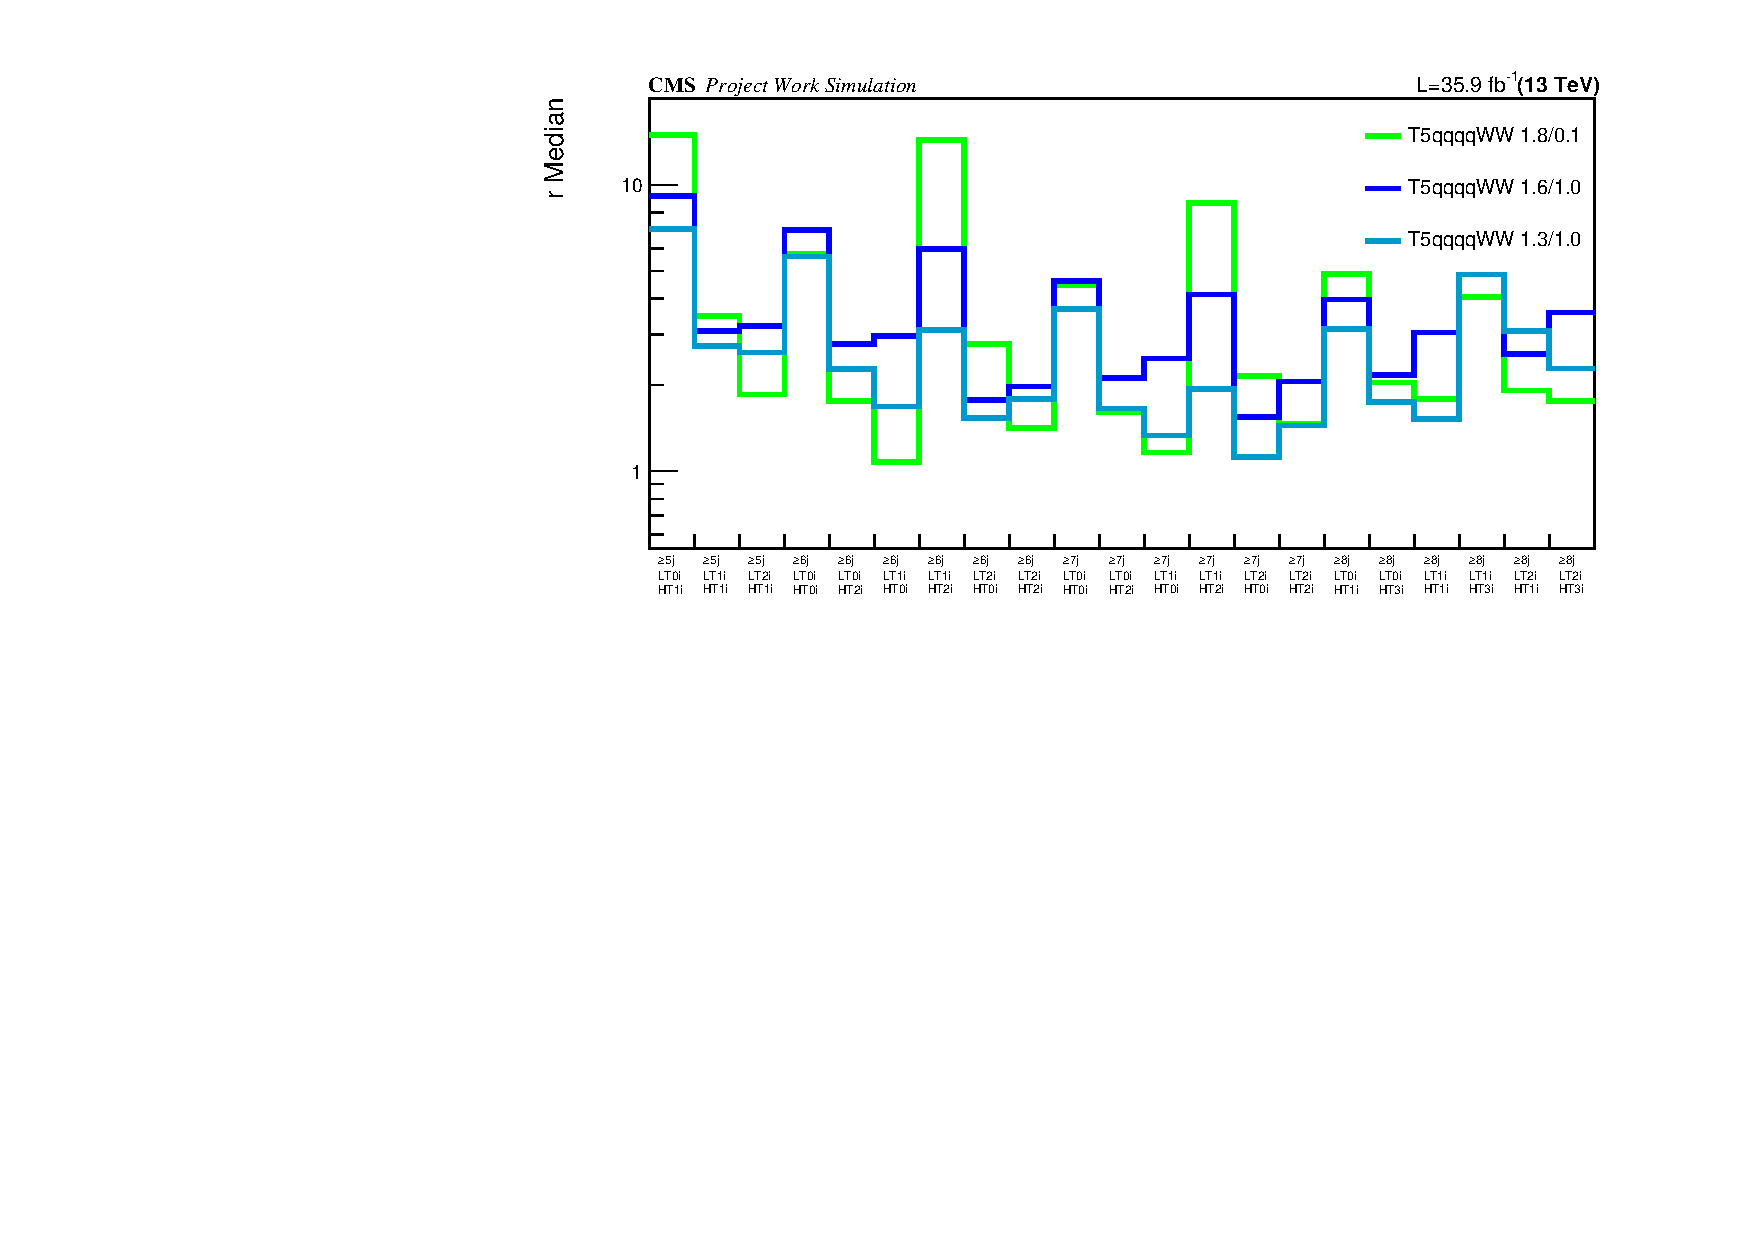
\includegraphics[width=0.95\textwidth]{PhD_Thesis_v4/Plots/analysis/signalRegions/r_valueperbin.pdf}
\end{center}
\caption{r-value calculated for each of the inclusive aggregate bins.}
\label{fig:rvalues}
\end{figure}

\begin{table}[ht]\begin{center}
\caption{Simulation table of the aggregate signal regions, 35.9~fb$^{-1}$}\label{tab:Aggrsim_results}
\resizebox{\textwidth}{!}{\begin{tabular}{c|c|c|c|l|rrr|rrr|rrr|rrr|}\hline
 \multirow{2}{*}{\njet}     & \LT & \DF & \HT     & \multirow{2}{*}{Bin name} & \multicolumn{6}{c|}{T5qqqqWW $m_{gl}$/$m_{\ninozero}$ $[$TeV$]$} & \multicolumn{3}{c|}{tot. background} \\%\hline
 & $[$GeV$]$&[rad] &$[$GeV$]$ &   & \multicolumn{3}{c}{(1.5/1.0)} & \multicolumn{3}{c|}{(1.9/0.1)} & \multicolumn{3}{c|}{Simulation}  \\\hline
\hline
\multirow{1}{*}{$\geq5$}
&\multirow{1}{*}{$\geq650$}&0.5
&$\geq750$
 & $\textrm{LT2i},  \textrm{HT1i}$
 & 6.15&$\pm$&0.57 & 6.29&$\pm$&0.2 & 20.24&$\pm$&1.27
 &  \\
\cline{2-14}
\hline
\hline
\multirow{2}{*}{$\geq6$}
&\multirow{1}{*}{$\geq450$}&0.75
&$\geq500$
 & $\textrm{LT1i},  \textrm{HT0i}$
 & 16.59&$\pm$&0.94 & 5.28&$\pm$&0.19 & 31.22&$\pm$&1.55
 &  \\
\cline{2-14}
&\multirow{1}{*}{$\geq650$}&0.5
&$\geq1000$
 & $\textrm{LT2i},  \textrm{HT2i}$
 & 4.01&$\pm$&0.46 & 4.98&$\pm$&0.18 & 6.53&$\pm$&0.71
 &  \\
\cline{2-14}
\hline
\hline
\multirow{2}{*}{$\geq7$}
&\multirow{1}{*}{$\geq450$}&0.75
&$\geq500$
 & $\textrm{LT1i},  \textrm{HT0i}$
 & 9.47&$\pm$&0.71 & 3.54&$\pm$&0.15 & 10.97&$\pm$&0.86
 &  \\
\cline{2-14}
&\multirow{1}{*}{$\geq650$}&0.5
&$\geq500$
 & $\textrm{LT2i},  \textrm{HT0i}$
 & 4.28&$\pm$&0.48 & 3.3&$\pm$&0.15 & 4.28&$\pm$&0.59
 &  \\
\cline{2-14}
\hline
\hline
\multirow{1}{*}{$\geq8$}
&\multirow{1}{*}{$\geq250$}&1.0
&$\geq1250$
 & $\textrm{LT0i},  \textrm{HT3i}$
 & 1.82&$\pm$&0.31 & 1.71&$\pm$&0.11 & 7.85&$\pm$&0.73
 &  \\
\cline{2-14}
\hline\end{tabular}}\end{center}\end{table}

